\chapter{Marco referencial}
\label{chap:FrameworkOfReference}

\section{Marco conceptual}
\label{Sec:FrameConcepts}

    \subsection{Inteligencia artificial}
    \label{sub:FrameAI}
    
        ``\textit{El estudio de cómo producir máquinas que tengan algunas de las cualidades que tiene la mente humana, como la capacidad de comprender el lenguaje, reconocer imágenes, resolver problemas y aprender.}'' \cite{CambridgeDicAI}. \\ 
    
        La inteligencia artificial (I.A.) es una de esas ciencias que ha acompañado a la humanidad por un largo tiempo, o al menos el deseo de ella y ciertamente las herramientas requeridas que pueden datar de milenios. La I.A. une conceptos con origen tan distantes en el tiempo como la lógica de los antiguos griegos, o la moderna computación. También materias que en principio parecen de aplicación tan lejana como la filosofía y la neurociencia, además de muchas otras como la algoritmia, la lingüística, las ciencias de la información y hasta la evolución natural. Todo en un mezcla maravillosamente engranada como una de las más grandes proezas de la la humanidad.
        
        Hoy en día se reconoce la lógica silogística de Aristóteles como uno de los primeros intentos de identificar bases cómo funciona el cerebro humano de manera estructurada y por medio de un conjunto de reglas, silogismos, que describen una parte del funcionamiento de la mente humana. Muchos más avances en el entendimiento de la mente fueron necesarios, entre ellos la propuesta de René Descartes, para explicar a los animales como máquinas complejas. 
        
        Pero también fue necesario del desarrollo de máquinas como la primera calculadora creada por Blaise Pascal, posteriormente mejorada por Leibniz. Así mismo la creación de autómatas muy sofisticados para cada época, siempre han sidos relacionados con la inteligencia, en el siglo XVIII el relojero Pierre Jaquet-Droz creo algunos que aun hoy impresionan por su nivel d detalle y precisión como el escritor, el dibujante o el músico, actualmente expuestos en el museo de arte e historia de Neuchâtel en suiza.
        
        Sin duda una de las bases fundamentales de los sistemas de computación actual desde el punto de vista matemático es el aporte que hizo George Boole con el establecimiento de la lógica proposicional o lógica booleana, pocas décadas después extendida por Gottlob Frege.
        
        El siglo XX fue sin duda, el siglo en que todos los avances tanto filosóficos, matemáticos y técnicos se juntaron para dar nacimiento a lo que actualmente se conoce como inteligencia artificial, si bien es cierto que aun no existe una definición completamente uniforme.
        
        Hacia la década de los veinte del siglo pasado el escritor Gottlob Frege acuño el término Robot para referirse a autómatas pseudo inteligentes que reemplazarían el al ser humano en el trabajo. Término que hoy se usa muy frecuentemente en el campo de la informática, y de la automatización en general, y al que la ciencia ficción suele atribuir inteligencia similar sino superior a la humana.
        
        En el año 1936 Alan Turing estableció las bases teóricas de la computación, lo que posteriormente llevo al concepto de máquina de Turing. Una máquina que conceptualmente podría realizar operaciones a partir de instrucciones escritas en una cinta, lo que terminaría por convertirse en el precursor de los ordenadores actuales.
        
        Generalmente el trabajo de Warren McCulloch y Walter Pitts en 1943 \cite{McCulloch1943} es considerado como el primero en el campo de la inteligencia artificial. Ellos basaron su trabajo en fisiología básica, la función de las neuronas en el cerebro y la lógica proposicional. 

        Antes de que las definiciones sobre qué es inteligencia artificial, se hicieran más o menos homogéneas, el gran Allan Turing planteó un problema que serviría como referente para poder establecer si una máquina era inteligente o no. En 1950 Turing en su artículo 'Computing Machinery and Intelligence', publicó el conocido test de Turing \cite{Turing1950} que, en términos generales, planteaba la posibilidad de establecer una conversación, usando un canal indirecto, entre una máquina y una persona sin que ésta ultima pudiera discernir si su interlocutor era también un ser humano o no. 
        
        En 1958, John McCarthy inventa LISP, el primer lenguaje para inteligencia artificial. Ese mismo año Rosenblatt presentó el 'Perceptrón'\index{Perceptrón} \cite{Rosenblatt1958}, un concepto inspirado en las redes neuronales del cerebro animal.
        
        La pregunta fundamental planteada por Turing: ¿puede pensar una máquina? ha llevado a diferentes definiciones sobre qué es el pensamiento y qué es la inteligencia.
        
        ``\textit{La automatización de actividades que asociamos con el pensamiento humano, actividades como la toma de decisiones, la resolución de problemas, el aprendizaje ...}'' \cite{Bellman1978}. \\
        
        Durante la segunda mitad del siglo XX se propusieron diferentes técnicas y algoritmos en el campo de la inteligencia artificial: Sistemas expertos, algoritmos genéticos, entre otros y también se crearon lenguajes de programación como Lisp y Prolog. Así mismo nuevas definiciones sobre qué es la I.A. han sido planteadas.
        
        ``\textit{La teoría y el desarrollo de sistemas informáticos capaces de realizar tareas que normalmente requieren inteligencia humana, como la percepción visual, el reconocimiento de voz, la toma de decisiones y la traducción entre idiomas.}'' \cite{OxfordDicAI}. \\
        
        ``\textit{La inteligencia artificial (IA) es una disciplina académica relacionada con la teoría de la computación cuyo objetivo es emular algunas de las facultades intelectuales humanas en sistemas artificiales.}'' \cite[Pag. 12]{benitez2014AI} \\
        
        Por su parte, Stuart Russell y Peter Norvig dividen la inteligencia artificial en seis disciplinas \cite{Russell2009}: 
        
        \begin{itemize}
            \item \textbf{procesamiento del lenguaje natural} para permitirle comunicarse con éxito.
            \item \textbf{Representación del conocimiento} para almacenar lo que sabe o escucha.
            \item \textbf{Razonamiento automatizado} para usar la información almacenada para responder preguntas y sacar nuevas conclusiones.
            \item \textbf{Aprendizaje automático} para adaptarse a nuevas circunstancias y detectar y extrapolar patrones.
            \item \textbf{Visión por computadora} para percibir objetos, y
            \item \textbf{robótica} para manipular objetos y moverse.
        \end{itemize}
  
        A partir de las diferentes definiciones es posible enmarcar a la inteligencia artificial como la capacidad que se brinda a un ordenador u otra máquina para realizar acciones que requieren inteligencia. Entre estas acciones están la capacidad de tomar decisiones basadas en la experiencia aun con información insuficiente o conflictiva, la capacidad de comprender el lenguaje humano y la capacidad de reconocer patrones en un conjunto de datos dado.
    
    \subsection{Aprendizaje automático (Machine learning)\index{Machine learning}}
    \label{sub:FrameMachineLearnig}
        
        ``\textit{Campo de estudio que provee a los ordenadores la habilidad de aprender algo sin ser explícitamente programado.}''. \cite{Samuel1959}.  (Traducción propia).
        
        \textbf{- ¿Qué es aprender? -} ``\textbf{Aprendizaje} es un término muy general que denota la forma, o formas, en la cual un animal (o una máquina) aumenta su conocimiento y mejora sus capacidades de actuación ('performance') en un entorno. De esta manera, el proceso de aprendizaje puede ser visto como un generador de cambios en el sistema que aprende - que por otra parte ocurren lentamente, adaptativamente - y que pueden ser revocados o ampliados.'' \cite[Pág. 6]{Moreno1994aprendizaje}.
        
        El Aprendizaje automático (en inglés Machine learning)\index{Machine learning} también conocido como aprendizaje de máquina, es una rama de la Inteligencia artificial \index{Inteligencia artificial} que conociste, de forma simplificada, en la creación de algoritmos que permiten dotar a los ordenadores con la capacidad de realizar tareas para la cuales no fueron explícitamente programados, es decir, aprenden de forma automática. 
        
        En un sentido más generalista para el campo del aprendizaje automático, es válido decir que un sistema debe aprender a separar la señal del ruido en los datos, de forma que se construya un engrama \index{Engrama} o  modelo que se ajuste más acertadamente al patrón en los datos.
            
        Los modelos generados en el aprendizaje automático son esencialmente paramétricos y el conocimiento se sustenta en el ajuste del valor de los parámetros. Es en la etapa de entrenamiento donde se ajustan los parámetros del modelo y es justo aquí donde la asociación o generalización de un comportamiento (salida) se asocia con el estimulo recibido (entrada).
        
        Así pues, en este contexto, el aprendizaje automático consiste en la identificación de patrones a partir de una muestra de datos de entrenamiento\index{Dataset}. Durante la etapa de entrenamiento, los sistemas que utilizan técnicas de aprendizaje automático, son capaces de tomar los datos y extraer de ellos las características intrínsecas de los mismos, de forma que puedan predecir comportamientos futuros para datos no observados mientras se realizo el entrenamiento. De igual forma, el Machine learning\index{Machine learning} implica mejoramiento del sistema sin la intervención humana.
        
        ``\textit{Se puede decir que un programa aprende a partir de la experiencia 'E', respecto a una tarea 'T' y alguna medida de rendimiento 'P', si el rendimiento en 'T', medido por 'P', mejora con experiencia 'E'.}'' \cite{Mitchell1997}. (Traducción propia). \\
        
        El Aprendizaje automático \index{Machine learning} se encuentra presente hoy día en todos los sistemas de entretenimiento o venta en línea, de relevancia mundial, como pueden ser las recomendaciones de productos en la tienda de Amazon o de contenido en la plataforma Netflix. Pero incluso en los asistentes virtuales de los teléfonos móviles u otros como el dispositivo Google Home, Alexa o Siri utilizan las técnicas de Machine learning\index{Machine learning} para que el comportamiento de estos asistentes sea cada vez más cercano a la persona que los usa, así por ejemplo, en el reconocimiento de comandos por voz puede ir aprendiendo la forma en que una determinada persona pronuncia algunas palabras he incluso la intención o emoción como las dice.
        
        En conclusión se podría decir que Machine learning\index{Machine learning} es un maestro del reconocimiento de patrones que, a partir de un conjunto de datos es capaz de inferir las reglas que intrínsecas, para que un ordenador aprenda de los mismos, sin la necesidad de que un humano defina y programe dichas reglas de forma explicita en un software, dotándolo con esto, además, de la capacidad de adaptase a los propios datos e incluso cambiar con el tiempo sin intervención humana.
    
    \subsection{Aprendizaje supervisado}
    \label{sub:FrameSupervisedLearnig}
    
        ``\textit{En el aprendizaje supervisado, el objetivo es aprender un mapeo de la entrada a una salida cuyos valores correctos son proporcionados por un supervisor.}'' \cite[Pág. 11]{alpaydin2014ML} (Traducción propia).\\
        
        El aprendizaje supervisado es una técnica dentro del aprendizaje automático\index{Machine learning} que permite deducir la función que mejor se ajusta a una muestra de vectores emparejados Entrada-Salida, es decir, ajustar los parámetros de un modelo de forma que éste permita tomar la entrada, ejecutar el conjunto de operaciones dentro del sistema y obtener valores que se acerquen lo más posible a la salida esperada. 
        
        En otras palabras, cuando se entrena un sistema, usando la técnica aprendizaje supervisado, se tiene un conjunto de datos de ejemplo (ver sección \ref{Sec:FrameDataset} para mayor detalle sobre Datasets\index{Dataset}) $x[0, 1, ..n]$ correspondientes a las entradas al sistema y un conjunto de salidas correspondientes $y[0, 1, ..n]$ donde cada entrada del vector $x$ se asocia con una salida del vector $y$. El objetivo del aprendizaje supervisado es encontrar la función que permita generalizar los datos (modelo), de forma que, en un futuro, se pueda predecir el valor de salida correspondiente a cualquier entrada sin que haya visto dicha entrada durante el entrenamiento.
        
        Debido a la naturaleza misma de este algoritmo, es necesario contar con un conjunto de datos suficientemente amplio para establecer la generalización, además la correcta etiquetación de cada dato de entrada con su salida correspondiente, de no ser así, se podrían generar un modelo de predicción poco confiable o que el aprendizaje nunca se dé. Es por esto que la preparación de los datos, constituye uno de los pasos fundamentales de este tipo de aprendizaje, siendo incluso el que consuma gran parte del tiempo en la construcción del sistema.
        
        En el aprendizaje supervisado se suelen separar los modelos generados en dos categorías, dependiendo el tipo de salida obtenida: por un lado están los modelos de clasificación, que permiten obtener un valor que pertenece a un conjunto de posibles valores. Y por otro lado, los modelos de regresión, cuya salida es un valor de un espacio continuo.
        
        Algunos de los ejemplos más notorios dentro de la Inteligencia artificial\index{Inteligencia artificial} de métodos de aprendizaje supervisado son: Regresión logística, SVM\index{SVM}, Redes neuronales\index{Redes neuronales}, Árboles de decisión entre otros. 
    
    \subsection{Aprendizaje no supervisado}
    \label{sub:FrameNoSupervisedLearnig}
        
        ``En el aprendizaje no supervisado, no existe tal supervisor y solo tenemos datos de entrada. El objetivo es encontrar las regularidades en la entrada.'' \cite[Pág. 11]{alpaydin2014ML} (traducción propia).\\
        
        El aprendizaje no supervisado es un método de entrenamiento dentro del campo del aprendizaje automático\index{Machine learning} que permite, a partir de un conjunto de datos\index{Dataset} sin etiquetas a priori, identificar las características de los elementos de la muestra,  es decir, sin saber cual es la salida esperada, generar un modelo de densidad que permita caracterizar o agrupar los datos.
        
        Un uso habitual de este tipo de métodos es la segmentación de conjuntos de datos por atributos compartidos, este uso está muy extendido dentro de los denominados 'recomendadores', algoritmos que permiten, por ejemplo, encontrar usuarios con gusto similares y así poder recomendar productos o contenidos que también han sido adquiridos por otros miembros de la misma categoría. Un ejemplo de este tipo de métodos es el algoritmo K-means que permite crear agrupaciones a partir de la cercanía de las características de los datos.
        
        Otro uso habitual es detección de anomalías que no encajan en ningún grupo, por ejemplo la identificación de células cancerosas \cite{kakushadze2017}. Pero también pueden ser usadas para la simplificación de conjuntos de datos, agrupando elementos con atributos similares, esto tiene especial utilidad, cuando el coste de preparar los datos (etiquetar) es muy alto o se desconoce la salida esperada.
        
        Por tanto, se puede decir que esta técnica busca identificar la estructura intrínseca de los datos. En el aprendizaje no supervisado se suelen separar los modelos generados en dos categorías, dependiendo el tipo de salida obtenida:
        agrupación y reducción de la dimensionalidad.
        
    \subsection{Aprendizaje reforzado\index{Aprendizaje reforzado}}
    \label{sub:FrameReinforcementLearning}
        
        ``\textit{Un proceso de prueba y error basado en recompensas, en el que un sistema aprende a interactuar con un entorno complejo para lograr resultados gratificantes, se conoce en lenguaje de aprendizaje automático como aprendizaje de refuerzo. En el aprendizaje por refuerzo, el proceso de prueba y error es impulsado por la necesidad de maximizar las recompensas esperadas a lo largo del tiempo.}'' \cite[Pág 374]{Aggarwal2018} (traducción propia).\\

        En I.A. se espera que un sistema que cuenta con aprendizaje automático\index{Machine learning} 'aprenda' a tomar las decisiones correctas, incluso en situaciones cambiantes. Por ejemplo, cuando se trata de vehículos autónomos, en estos casos es natural suponer que no se puede contar, a priori, con la secuencia de acciones correctas a realizar debido principalmente a la gran cantidad de variaciones que el propio entorno puede tener. Con esto es difícil modelar las acciones del sistema debido a que debe ser una secuencia de acciones dinámicas. 
        
        ``\textit{La suposición clave aquí es que estos sistemas son demasiado complejos para modelar explícitamente, pero son lo suficientemente simples como para evaluarlos, de modo que valor de recompensa se puede asignar para cada acción.}'' \cite[Pág 44]{Aggarwal2018} (traducción propia).\\
        
        En forma general se puede decir que el aprendizaje reforzado consiste en un mecanismo en el que un agente va adaptando su comportamiento tras cada acción que realiza, mediante la recompensa (o castigo). Es decir, si una acción en concreto es beneficiosa dentro del objetivo general se otorga un puntaje, de esta forma, se va construyendo la política de acción. Un ejemplo de este tipo de aprendizaje es algoritmo Q-learning\index{Q-learning}.
        
        ``Un buen ejemplo es un videojuego, donde un solo movimiento por sí solo no es tan importante; sino que es la secuencia de movimientos correctos lo que lo hace bueno. Un movimiento es bueno si es parte de una buena política de juego.''  \cite[Pag. 13]{alpaydin2014ML} (Traducción propia).\\
        
        Los videojuegos durante los últimos años se han convertido en los entornos de pruebas para este tipo de algoritmos, pues presenta una gran variabilidad en un ambiente controlado y que justamente permite probar la premisa de 'Aprendizaje por recompensa'. Considerando el caso del clásico juego 'Pacman' en el el personaje central en cada momento del juego solo puede hacer una de cuatro posibles acciones, avanzar a la izquierda, a la derecha, arriba o abajo. Sin embargo, de la acción de realice en cada momento dependerá que reciba más punto o incluso pierda la partida. Al tomar en consideración los posibles estados en los que el personaje central esté en una de las posibles posiciones dentro del tablero de juego y los 'fantasmas' estén cada uno en su posición, genera una combinación de posibilidades tan grande que hace inviable definir las acciones a tomar en cada estado. Es aquí donde el aprendizaje por refuerzo permite identificar la mejor acción para cada estado, dependiendo la recompensa que reciba al realizar el movimiento. 
        
        Es importante considerar que este tipo de algoritmos no indican una 'verdad absoluta', en cuanto que la secuencia de movimiento es la mejor posible en un entorno, simplemente es una lo suficientemente buena para cumplir el objetivo.
    
    \subsection{Aprendizaje profundo (Deep learning)\index{Deep learning}}
    \label{sub:FrameDeepLearnig}
    
        Aprendizaje profundo (en inglés, Deep learning) es un conjunto de algoritmos dentro de la rama de Aprendizaje automático\index{Machine learning} que busca la generación de modelos que permitan inferencias de alto nivel a partir de grandes conjuntos de datos. Para esto hace uso de arquitecturas computacionales de múltiples capas, que realizan transformaciones no lineales y de forma iterativa a  los datos de entrada.
        
        ``La idea detrás de las arquitecturas profundas es que pueden aprovechar mejor las regularidades repetidas en los patrones de datos para reducir el número de unidades computacionales y, por lo tanto, generalizar el aprendizaje incluso a áreas del espacio de datos donde no hay ejemplos.'' \cite[Pág 34]{Aggarwal2018}. (Traducción propia).\\
        
        El concepto de 'profundo' se debe esencialmente a la cantidad de transformaciones aplicadas, respecto de otros métodos de aprendizaje. Además, cada transformación cuenta con umbrales y pesos que son modificados durante el entrenamiento. Aunque no hay una definición clara de cuántas transformaciones son requeridas para poder ser llamado profundo, algunos de los modelos actuales dentro de esta categoría pueden superar el millón de parámetros entrenables.
        
        ``\textit{Un MLP (Perseptrón multicapa) con una sola capa oculta tiene una capacidad limitada, mientras que el uso de un MLP con múltiples capas ocultas puede aprender funciones más complicadas de la entrada. Esa es la idea detrás de las redes neuronales profundas donde, a partir de la entrada sin procesar, cada capa oculta combina los valores en su capa anterior y aprende funciones más complicadas.}'' \cite[Pág 307]{alpaydin2014ML}. (Traducción propia).\\
        
        La profundidad misma, es decir, el número de transformación trae consigo un problema implícito, éste es el desvanecimiento gradual de la relevancia de los datos de entrada, pues su transformación acumulada es tan alta, que el impacto de los parámetros entrenables es mayor que el de los propios datos de entrada, consiguiendo, con esto, que la relevancia de la entrada se pierda a medida que se aumenta la profundidad, convirtiéndose en un sistema esencialmente determinista. Para subsanar el problema del desvanecimiento gradual, se han planteado diferentes estrategias (ver \ref{sub2:GradientVanishing}) y también se han definido arquitecturas como las redes residuales \cite{Kaiming2015} (ver \ref{sub:FrameResNet}).
        
    \subsection{Redes neuronales (NN)}
    \label{sub:FrameNeuralNetworks}
    
        \subsubsection{Breve historia}
        \label{sub2:History}
 		
            En el año 1943 Warren McCulloch y Walter Pitts presentaron un primer modelo para la creación de redes neuronales artificial \cite{McCulloch1943}, partiendo de tres fuentes: El conocimiento existente sobre el funcionamiento de las las neuronas del cerebro y su fisiología, el análisis formal de la lógica proposicional de Russell y Whitehead y la teoría de la computación de Turing. Con esto presentaron un modelo constituido a su vez por modelos de neuronas artificiales, de forma que cada una de ellas pudiera ser representada como 'activada' o 'desactivada' a partir de los 'estímulos' (entrada / inputs) recibidos, siendo un modelo equivalente a las neuronas naturales. Además mostraron que cualquier función podría computarse usando la red de neuronas interconectadas ya que pes posible con las estructuras de red propuestas, implementar las compuertas lógicas tradicionales: and, or, nor o cualquier otra. Este modelo sentó las bases para los futuros desarrollos de redes para la inteligencia artificial.
            
            ``\textit{Se puede crear una red neuronal artificial simulando un modelo de una red de neuronas en un computador. Al aplicar algoritmos que imitan los procesos de las neuronas reales, es posible hacer que la red 'aprenda' a resolver muchos tipos de problemas.}'' \cite{Krogh2008}. \\
            
            Más adelante en 1949 Donald Hebb, publicó un a hipótesis sobre los mecanismos en que las neuronas interactúan para generar lo que se conoce como aprendizaje. Hebb a partir de sus estudios (entre los que se encuentran el estudio de la sinapsis basado en el famoso experimento de Pavlov) entendió, entre otras cosas, que una neurona no era capaz, por si sola, de excitar a otra, pero que el acto conjunto de varias si podría desencadenar en la activación o desactivación. Además plantea el modelo que define la plasticidad del cerebro:
            
            ``\textit{Si las entradas a un sistema producen el mismo patrón de actividad repetidamente, el conjunto de elementos activos que constituyen ese modelo llegarán a tener una interasociación más fuerte. Es decir, cada elemento tenderá a activar a otros elementos y (con pesos negativos) a inactivar a los elementos que no formen parte del patrón. En otras palabras, el patrón en su conjunto se convertirá en 'auto-asociado'. Se puede decir que un aprendizaje (auto-asociado) es un patrón de engrama.}'' \cite{Hebb1949}. \\
            
            De la hipótesis de Hepp se desprendió uno de los conceptos más tradicionales en el campo de la inteligencia artificial, el aprendizaje no supervisado. En poco tiempo algunos investigadores empezaron a aplicar las ideas de Hebb en el ámbito computacional. En 1954 Farley y Clark \cite{Farley1954} construyeron un experimento para simular una red con los conceptos de Hepp usando máquinas computacionales. En 1958 Rosenblatt presento el 'Perceptrón'\index{Perceptrón} \cite{Rosenblatt1958}, un algoritmo para el reconocimiento de patrones, basado en sus ideas de como la información acerca del mundo físico es almacenada e interpretada y como esa información influencia el reconocimiento de las cosas.
            
            A pesar de los avances alcanzados, por al menos una década, el desarrollo del campo de las redes neuronales se estancó, en gran medida por dos factores, en primera instancia por falta del poder computacional y en segunda instancia, por falta de algoritmos que permitieran el 'entrenamiento' del Perceptrón\index{Perceptrón}. Fue hasta que Paul Werbos presentó en 1975 su algoritmo de propagación hacia atrás \cite{Werbos1975} (Back propagation en inglés), que se logró una forma eficaz para el entrenamiento de las redes. El éxito de la propuesta de Werbos radica en utilizar la diferencia entre el resultado producido y el resultado deseado para cambiar los "pesos" de las conexiones entre las neuronas artificiales (Vea la sección \ref{sub:FrameBackPropagation}, para un mayor detalle de este algoritmo.).
            
            A pesar de la mejora en los algoritmos, el problema de poder computación siguió vigente hasta mediados de la década de los 2000, cuando se empezaron a alcanzar capacidades de computo más acordes a las necesidades, así mismo se pudo desarrollar redes cada vez más grandes. Y dada la naturaleza altamente paralelizable en el procesamiento de las redes neuronales, un nuevo avance en el poder de computo se logró tras la inclusión de las tarjetas de vídeo (GPU) en el procesamiento.
            
            Actualmente las redes neuronales están siendo usados por investigadores de diferentes áreas, no solo donde los algoritmos tradicionales son poco efectivos, sino también en la solución de nuevos problemas como la detección de exo-planetas \cite{NasaExoplanet2017}. 
            
        \subsubsection{Definición técnica}
        \label{sub2:TecnichialNN}
        
 		    ``\textit{Una red neuronal artificial (ANN) es un modelo computacional que está ligeramente inspirado en el cerebro humano, ya que consiste en una red interconectada de unidades de procesamiento simples (neuronas artificiales) que aprenden de la experiencia al modificar sus conexiones.}'' \cite{VanGerven2017}. \\
        
            De forma general se puede decir que las redes neuronales son un modelo parámetrico, es decir, la representación matemática de un proceso o fenómeno con el cual se puedan realizar predicciones. En otras palabras, a partir de un conjunto $x$ de valores de entrada es capaz de inferir un conjunto $y$ de valores de salida. 
            
            De forma esquemática, las redes neuronales artificiales las neuronas están dispuestas en capas y, a su vez, cada capa está compuesta por nodos (neuronas), donde los párametros de entrada de una capa corresponden con los valores de salida de la capa inmediatamente anterior, (algunas arquitecturas pueden diferir en algunas pares de esta premisa, ver sección \ref{sub2:FrameNNArchitecture}). Según su ubicación en la red, cada capa pertenece a una de los siguientes grupos: entrada, salida o capas ocultas, como se ve en la figura \ref{fig:GeneralNN}.
            
            \begin{figure}[ht!]
            	\centering
            	\includegraphics[width=0.6\linewidth]{imgs/02-Referential/02-GeneralNN.png}
            	\caption[Modelo general de una red neuronal]{Modelo general de una red neuronal.}
        	    \label{fig:GeneralNN}
            \end{figure}%
            
            Antes de presentar el como se transmite o fluyen los datos en la red desde la entrada hasta la predicción, considere cada nodo o neurona de la red como el resultado de la ecuación \ref{EQ:BasicNeuron}.
            
            \begin{equation}
                \label{EQ:BasicNeuron}
                y = f(b + \sum_{i=0}^n w_i x_i)
            \end{equation}
            
            Donde $y$ es el valor de salida de la neurona, $f$ es una función de activación \index{Función de activación} (vea \ref{sub:FrameActivationFunctions} para mayor detalle), $x$ el conjunto valores de entrada, $w$ el conjunto de parámetros que ajustan el peso o importancia que tiene cada valor del conjunto $x$. Finalmente, $b$ es un valor de sesgo que se aplica a la neurona misma, este sesgo se suele considerar como la conexión con otra neurona cuya salida siempre será $1$.
            
            La red neuronal más simple es el Perceptrón \index{Perceptrón} (ver figura \ref{fig:Perceptron}). Ésta es simplemente una red de un única capa, esto se considera así, pues a los valores que recibe la capa de entrada no se aplica ningún ajuste sino que son transmitidos directamente a la siguiente capa.
            
            \begin{figure}[ht!]
            	\centering
            	\includegraphics[width=0.6\linewidth]{imgs/02-Referential/02-Perceptron.png}
            	\caption[Modelo del Perceptrón]{Modelo del Perceptrón.}
        	    \label{fig:Perceptron}
            \end{figure}%
            
             A pesar de que un Perceptrón \index{Perceptrón} cuenta con todas las características fundamentales de una red neuronal, su limitada cantidad de parámetros no permite su aplicación a problemas con más dimensiones como es el caso de la clásica compuerta $Xor$, en su lugar se suelen usar redes con un número mucho más amplio de capas y de neuronas como se muestra en la figura \ref{fig:PerceptronMulti}, esto es conocido como el 'Perceptrón multicapa' \index{Perceptrón multicapa}. 
            
            \begin{figure}[ht!]
            	\centering
            	\includegraphics[width=0.6\linewidth]{imgs/02-Referential/02-PerceptronMulticapa.png}
            	\caption[Modelo del Perceptrón multi capa]{Modelo del Perceptrón multi capa.}
        	    \label{fig:PerceptronMulti}
            \end{figure}%
            
        \subsubsection{Flujo de datos en la red}
        \label{sub2:FrameNNDataFlow}
            
            El flujo de datos de la red consiste en tomar los valores de entrada $x$ e ir pasándolos de una capa $c$ a la siguiente $c + 1$ hasta legar a la salida $y$, aplicando para cada neurona la ecuación \ref{EQ:BasicNeuron}, para eso, las redes neuronales hacen uso del algoritmo de 'propagación hacia adelante'\index{Forward propagation} (puede ver este algoritmo en detalle en la sección \ref{sub:FrameForwardPropagation}). 
            
            Por otro lado, el objetivo fundamental de las redes neuronales, como de cualquier otro algoritmo de aprendizaje automático es reducir el error o lo también se conoce como función de pérdida \index{Función de pérdida} (remítase a la sección \ref{sub:FrameLossFunction} para mayor detalle sobre las funciones de pérdida). Para reducir el error se ajustan los parámetros $w$ y $b$ es decir, se cambia la influencia de cada entrada respecto a la diferencia entre el valor de salida obtenido y el valor esperado. Cuando se habla de valor esperado, se remite específicamente al conjunto de valores de entrenamiento de la red (ver sección \ref{Sec:FrameDataset} sobre conjuntos de datos de entrenamiento).
            
            Al cambiar los parámetros de cada neurona es justamente cuando ocurre lo que se conoce como 'aprendizaje'. Considere lo siguiente, cuando una red neuronal se crea los valores de $w$ y $b$ son asignados con valores aleatorios, esto es porque los pesos o influencia de cada $x$ no se conocen a priori y, por tanto, la salida obtenida también es un valor que no coincidirá con lo esperado. 
            
            Para que la red vaya aprendiendo es decir, que los parámetros se vayan ajustando de forma que la salida obtenida se acerque cada vez más a la esperada, se realiza el proceso conocido como entrenamiento, el cual se apoya de dos algoritmos principales: el 'descenso del gradiente' \index{Descenso del gradiente} (explicado en la sección \ref{EQ:GradientDescendent}) y la 'propagación hacia atrás' \index{Back propagation} (Explicado en la sección \ref{sub:FrameBackPropagation}).
            
            El 'descenso del gradiente', se encarga de encontrar el impacto del error acorde a la función de pérdida \index{Función de pérdida} utilizada, para encontrar un valor menor o que generé un menor error. Mientras que el algoritmos de 'propagación hacia atrás' se encarga de ir propagando el ajuste a los parámetros, acorde al resultado del descenso del gradiente, desde la capa de salida (la que tiene el valor final obtenido en la red), hacia las capas anteriores de forma iterativa. De esta forma se identifica el error y el impacto causado en cada nodo para generar dicho error y se va ajustando durante los múltiples ciclos en que se repite la 'propagación hacia atrás' durante el entrenamiento.
            
        \subsubsection{Arquitecturas de redes neuronales}
        \label{sub2:FrameNNArchitecture}
        
            \begin{figure}[ht!]
            	\centering
            	\includegraphics[width=0.8\linewidth]{imgs/02-Referential/02-NNZoo2019.png}
            	\caption[Listado de arquitecturas de redes neuronales]{Listado de arquitecturas de redes neuronales.}
        	    \label{fig:NNZoo2019}
            \end{figure}%
            
            La arquitectura de una red neuronal artificial es la forma o configuración como se organizan las neuronas en su interior, aunque también la forma en que el aprendizaje va llevarse a cabo. A lo largo del desarrollo de las redes neuronales se han propuesto diversas configuraciones, cada una con características propias y que presentan un ventajas según el campo utilizado pero también la forma en que aprenden. Dependiendo del problema puede ser más efectiva una u otra arquitectura de red. 
            
            Debido al éxito de algunas de las arquitecturas de las redes neuronales, varias de ellas han perdido el prefijo de arquitectura y se suele atribuir un nombre independiente, es decir como un tipo de red propia, sin embargo todas ellas siguen mantenido una estructura que incluye o depende del diseño original presentado anteriormente. Algunas de las arquitecturas más exitosas en las ultimas décadas son: las redes convolucionales (ver sección \ref{sub:FrameCNN}), las redes recurrentes (ver sección \ref{sub:FrameRNN}) y las redes residuales (ver sección \ref{sub:FrameResNet}), sin embargo, existe un conjunto muy amplió de arquitecturas, la figura \ref{fig:NNZoo2019} una recopilación de arquitecturas presentada por 'The Asimov Institute' \cite{NNZoo2019}.
        
    \subsection{Redes convolucionales (CNN)}
    \label{sub:FrameCNN}
    
        ``\textit{Las redes neuronales convolucionales han sido históricamente las más exitosas de todos los tipos de redes neuronales. Se utilizan ampliamente para el reconocimiento de imágenes, detección / localización de objetos e incluso procesamiento de texto.}'' \cite[Pág 41]{Aggarwal2018} (Traducción propia).
        
        Las redes convolucionales son un tipo de arquitectura de red neuronal. Puede ser considerada una adaptación a las redes neuronales tradicionales a las cuales se les adicionan capas de convolución. Las capas de convolución, son un modelo inspirado en el descubrimiento de Hubel y Wiesel sobre las células encargadas de la visión en gatos \cite{Hubel1962}, donde se hace inicialmente se identifican patrones simples como bordes y a medida que se avanza en las capas se van identificando características cada vez más complejas, a medida que se procesa la imagen. 
        
        La primera implementación de este modelo en el campo de la visión por computador fue hecha por Fukushima y Miyake en el trabajo que presentan el Neocognitron \cite{Fukushima1982}, mostrando la capacidad de modelo para tolerar variaciones. Sin embargo, solo fue hasta el trabajo de LeCun \cite{LeCun1998}, en los años 90, que se integró con el algoritmo de 'propagación hacia atrás' \index{Back propagation} pudiendo automatizar el aprendizaje de este tipo de capas.

        Las redes convolucionales han demostrado una superioridad sobre las redes tradicionales en cuanto a las exactitud de sus predicciones, principalmente en el campo de la identificación de patrones en imágenes, debido principalmente a una mayor tolerancia a variaciones. LeCun \cite{LeCun1998} demostró la eficacia de las redes convolucionales en el campo de la visión artificial tomando como caso de estudio la identificación de números escritos a mano. Para esto tomó un conjunto de imágenes de 28 x 28 píxeles en escala de grises. 
        
        Es importante considerar que el uso de imágenes hace el número de parámetros crezca muy rápido por ejemplo, para una imagen de 256x256 en escala de grises, se tendría en una capa tradicional 65.536 parámetros, o 3 veces ese valor si fuera una imagen RGB, para reducir la cantidad de parámetros es habitual poner capas con funciones de reducción como 'Max-pooling'\index{Max-pooling}. 
        
        Una ventaja de las redes convolucionales sobre las las tradicionales, consiste en que la entrada de una red tradicional debe mantener características homogéneas, es decir, mantener una disposición de los elementos en cada imagen con muy poca variación, lo cual normalmente no es fácil, un ejemplo de ello es el caso tomado por Lecun, donde es necesario superar las variaciones que tiene cada persona en su forma de escribir. 

        Las capas convolucionales se apoyan en que las imágenes tienen una rígida estructura en 2D, lo cual significa una fuerte correlación local de los datos, en otras palabras, el valor de un píxel depende y tiene estrecha relación con el valor de sus vecinos. Esto presenta una ventaja significativa, pues permite reconocer características simples, como bordes o esquinas, antes de intentar identificar características espaciales, lo que les permite su gran tolerancia a variaciones de desplazamiento, escala o distorsión.

        \subsubsection{Arquitectura habitual de una red convolucional}
            Normalmente una red convolucional está compuesta por varias capas de convolución a la entrada de la red, intercaladas con capas de reducción y posteriormente varias capas de red neuronal tradicional como se ve en la figura \ref{fig:ConvolutionArchitecture}.

            \begin{figure}[ht!]
            	\centering
            	\includegraphics[width=0.8\linewidth]{imgs/02-Referential/02-arch-cnn2.png}
            	\caption[Arquitectura tradicional de una red convolucional.]{Arquitectura tradicional de una red convolucional. }
        	    \label{fig:ConvolutionArchitecture}
            \end{figure}%
        
        \subsubsection{La convolución}
            El proceso realizado en una capa convolucional consiste en realizar una operación de producto punto entre una matriz llamado kernel y las submatrices de la imagen cuyo centro es cada uno de los píxeles de la imagen, haciendo un desplazamiento de izquierda a derecha y de arriba a abajo de la imagen, como muestra la imagen \ref{fig:ConvolutionSteps}, una vez realizada la multiplicación los valores obtenidos son sumados y pasado por una función de corrección no lineal (Típicamente ReLU\index{ReLU}, ver funciones de activación en la sección \ref{sub:FrameActivationFunctions}). 
            
            \begin{figure}[ht!]
            	\centering
            	\includegraphics[width=0.8\linewidth]{imgs/02-Referential/02-Convolution.png}
            	\caption[Pasos de una capa de convolución]{Pasos de una capa de convolución.}
        	    \label{fig:ConvolutionSteps}
            \end{figure}%
        
        \subsubsection{Relleno (Padding)}
            Es importante considerar que el desplazamiento de la matriz Kernel puede llevar a dos casos: primero, si el tamaño de las dimensiones del kernel es compatible con el tamaño de la matriz de entrada, es decir, cada dimensión de la matriz de entrada es múltiplo de su correspondiente en el kernel y, por tanto, el kernel podrá ir de inicio a fin sin que sobren elementos en una u otra. El problema de esto es que el kernel solo llegaría hasta el punto donde no exceda los bordes con lo que, en caso de una imagen se estaría perdiendo información de los bordes al no poder operar el kernel completamente.
            
            El segundo caso ocurre cuando las dimensiones de la matriz de entrada y del kernel no son compatibles, haciendo que queden elementos sobrantes. En el caso de una imagen podrían quedar píxeles sin analizar.
            
            \begin{figure}[ht!]
            	\centering
            	\includegraphics[width=0.4\linewidth]{imgs/02-Referential/02-Padding.png}
            	\caption[Capas de relleno para convolución]{Capas de relleno para convolución.}
        	    \label{fig:ConvolutionPadding}
            \end{figure}%
            
            Ninguno de de las dos pérdidas de información son deseables. Este problema se suele solventar con la adición de ceros antes y después de los límites de la matriz de entrada (ver fig. \ref{fig:ConvolutionPadding}), de forma que ambos problemas son solucionados, por una lado se asegura tener dimensiones compatibles entre las matrices y, además, extiende los limites para que el kernel pueda operar en su totalidad con todos los valores de la matriz de entrada. La adición de ceros no representa ninguna alteración a los datos de la matriz de entrada, debido a que al realizar el producto punto las operaciones generadas por el relleno no afectan el resultado.
            
        \subsubsection{Paso (Stride)}
            Un concepto adicional de las redes convolucionales es el \textbf{paso}. En lo mencionado anteriormente se describe un desplazamiento del kernel en el que solo se avanza un píxel antes de realizar la operación de convolución, sin embargo, esto también puede ser alterado para que dé dos o más saltos, aunque no se suele utilizar un numero muy alto para el desplazamiento, ya que se pierde granularidad. La ventaja. por otro lado, es que al aumentar el tamaño del paso se puede reducir el numero de operaciones y de valores resultantes para operar en la capa siguiente. 

        \subsubsection{Reducción (Pooling)}
            Las capas de reducción (Pooling \index{Pooling}) como el caso de Max-pooling\index{Max-pooling} permiten “quitar resolución” a la imagen, y así, tener menos parámetros que entrenar tras cada capa, permitiendo redes de mayor profundidad, es decir, más capas sin aumentar excesivamente las necesidades de cómputo, lo que a su vez otorga una mayor capacidad de aprendizaje a la red.
            
            El principio fundamental de este tipo de capas se conoce como sub muestreo (Sub-sampling), el cual toma solo algunos valores de un conjunto, por ejemplo, el Max-pooling\index{Max-pooling} toma submatrices y de estas extrae el mayor valor, de forma que luego de esta capa se tendrá una matriz de salida de tamaño reducido y con los máximos de cada sub matriz. Reduciendo enormemente los parámetros de entrada para la siguiente capa. Tal como se ve en el ultimo paso de la imagen \ref{fig:ConvolutionSteps}.

        \subsubsection{Entrenamiento de una red convolucional}
            El entrenamiento de aplicado a una red convolucional es esencialmente igual realizado en una red tradicional. Se hace uso del algoritmo Back propagation\index{Back propagation}, aunque también puede ser vista como la transpuesta de la convolución aplicada durante la etapa de predicción realizada con el algoritmo Forward propagation\index{Forward propagation}. Ambos, Forward Propagation y Back propagation son explicados en las secciones \ref{sub:FrameForwardPropagation} y \ref{sub:FrameBackPropagation} respectivamente.
            
    \subsection{Redes recurrentes (RNN)}
    \label{sub:FrameRNN}
    
        El análisis de imágenes puede ser hecho de forma integral ya que no es necesario tener otras imágenes para, por ejemplo, identificar objetos en ella, si bien es cierto que la existe una fuerte correlación entre los datos de la imagen (los píxeles), la información en su totalidad está contenida en la imagen, de esta forma un red neuronal puede recibir en un solo momento todos los datos necesarios para el análisis.
        
        A diferencia del análisis integral de las imágenes, tanto en la naturaleza como en el día a día de las personas, existen situaciones en que una acción depende del análisis de una secuencia de datos que tienen una estrecha relación unos de otros pero que ocurren en momentos diferentes. En otras palabras que un único momento no permite el correcto análisis del sistema. Algunos ejemplos de estos tipos de secuencias de datos son:
        
        \begin{itemize}
            \item \textbf{Las secuencias de tiempo}: un ejemplo de este tipo de secuencias es el análisis del clima, donde un estado $n+1$ está estrechamente relacionado con el estado $n$ y éste a su vez depende del estado $n-1$. Este puede ser el caso del reconocimiento del habla como los sistemas que convierten voz a texto.
            
            \item \textbf{Los textos}: Los textos son un ejemplo común de dependencia de estados, que una red neuronal tradicional no puede abordar correctamente. Esto se debe, no solo a la dependencia entre las palabras sino, además, porque no se conoce a priori la longitud de la frase a analizar. 
            
            Cuando se procesa un texto se podría pasar toda la frase a la red neuronal, sin embargo, el problema aquí radica en que no es posible definir el tamaño de la entrada, podría crearse una red que reciba, por ejemplo, diez palabras pero si la frase es más larga que eso se estaría perdiendo información y, por otro lado, si la frase es más corda quedarían entradas sin asignar.
            
            \item \textbf{Información genética}: El ADN de los seres vivos en nuestro planeta está compuesto por solo cuatro bases nitrogenadas, sin embargo, la combinación, el orden y la posición de cada una permiten codificar todas las instrucciones de generación de proteínas en las células, por tanto, es claro que el análisis de un solo par de bases no es suficiente, e incluso el de un único gen.
            
        \end{itemize}
        
        Considerando lo anterior se hace evidente que es necesario contar con una arquitectura de red que permita recibir un número de parámetros variable y que además mantenga la correlación entre ellos a los largo del tiempo.
        
        Las redes neuronales recurrentes (RNN)\index{Redes neuronales recurrentes}, son una arquitectura que contiene ciclos de forma que la salida de una neurona en un tiempo $(Y_t)$ se use como entrada en un momento posterior $(X_{t+1})$, generando con esto bucles de retroalimentación. La figura \ref{fig:RNN-basic} muestra el diseño general de este tipo de redes.
            
        \begin{figure}[ht!]
        	\centering
        	\includegraphics[width=0.6\linewidth]{imgs/02-Referential/02-arch-rnn-general.png}
        	\caption[Diseño general de una RNN]{Diseño general de una RNN.}
    	    \label{fig:RNN-basic}
        \end{figure}%
        
        El concepto de redes recurrentes apareció en los años 80s con los trabajos John J. Hopfweld \cite{Hopfield1982RNN}, posteriormente Jeffrey Elman presentó un modelo más generalista \cite{Elman1990RNN}. El principal impacto de las RNN\index{Redes neuronales recurrentes} consiste en que al almacenar información para utilizarla en momentos posteriores, a cuando se generó, con esto es posible decir que tiene memoria. Permitiendo con esto, el análisis de series de datos temporales. 
        
        \subsubsection{Entrenamiento de una RNN}
            Una RNN puede ser descrita como se muestra en la ecuación \ref{EQ:BasicRNN}:
        
            \begin{equation}
                \label{EQ:BasicRNN}
                y_t = f(Wx_t + Uy_{t-1} + b)
            \end{equation}
            
            Siendo $x=[x_1,x_2,x_n]$ la secuencia de entrada proveniente de una capa anterior, $W$ el peso aplicado a cada elemento de $x$. $y_{t-1}$ corresponde a la salida obtenida en un tiempo anterior y $U$ la matriz de pesos con los que se opera la salida del tiempo anterior. Finalmente, $b$ corresponde al sesgo propio de la neurona.
        
            En la etapa de entrenamiento de una RNN\index{Redes neuronales recurrente} se debe actualizar los pesos tanto en $W$ y $b$ como en $U$. Para esto se hace uso del algoritmo de Propagación hacia atrás (en ingles Back propagation)\index{Back propagation} (ver sección \ref{sub:FrameBackPropagation} para más detalle sobre Back propagation.
            
            El método de Back propagation\index{Back propagation} aplicado a las RNN cuenta con una variación por lo que se suele llamar propagación hacia atrás a través del tiempo (BPTT por sus siglas en inglés)\cite{Werbos1990BPTT}. Esté método incluye el concepto de desenrollar la red. Entendiendo que la recurrencia de este tipo de redes, se puede considerar como una red tradicional envuelta sobre sí misma y, de igual forma la dependencia de una capa respecto a las anteriores, como se ve en la figura \ref{fig:RNN-unfold}. 
            
            \begin{figure}[ht!]
            	\centering
            	\includegraphics[width=0.7\linewidth]{imgs/02-Referential/02-arch-rnn-unfold.png}
            	\caption[RNN desenrollada]{RNN desenrollada.}
        	    \label{fig:RNN-unfold}
            \end{figure}%
            
            Así pues, al desenrollar la red, el entrenamiento puede realizarse de la misma forma que una red tradicional, tomando cada bucle de tiempo almacenado como una capa más.
            
        \subsubsection{Variación LSTM\index{LSTM}}
            
            Con lo mencionado en el entrenamiento de una RNN es entendible las implicaciones del desdoblamiento, en primer lugar, la gran cantidad de capas adiciones que se agregan, lo que además del proceso mismo de desenrollar la red aumentan los requerimientos computacionales, en consecuencia aumenta el tiempo de entrenamiento.
            
            La segunda implicación, inherente a las redes y que se hace cada vez más notorio con el aumento de capas, es la explosión o el desvanecimiento del gradiente \cite{Hochreiter2001gradient} (ver la sección \ref{sub2:GradientVanishing} para más detalle de este concepto), impidiendo el cambio de los pesos de las conexiones entre las neuronas eficazmente.
        
            Para solucionar el problema de desvanecimiento, en 1997 Sepp Hochreiter y Jürgen Schmidhuber presentaron un tipo de red recurrente llamada Long Short Term Memory (LSTM)\index{LSTM} \cite{Hochreiter1997}.
       
            Las LSTM\index{LSTM} se apoyan de una estructura llamada Células de memoria. Las Células de memoria contienen una estructura que consta de tres puertas: \textit{de olvido}, \textit{de entrada} y \textit{de salida}, que permiten gestionar lo que es información importante y se debe conservar y lo que debe ser 'olvidado', de esta forma mantiene durante largos períodos (momentos), fragmentos de información. El esquema general de las Células de memorias se muestra en la figura \ref{fig:RNN-lstm}.
            
            \begin{figure}[ht!]
            	\centering
            	\includegraphics[width=0.9\linewidth]{imgs/02-Referential/02-arch-rnn-lstm.png}
            	\caption[Esquema de un bloque de LSTM]{Esquema de un bloque de LSTM.}
        	    \label{fig:RNN-lstm}
            \end{figure}%
            
            \textbf{Puerta de olvido}: Esta puerta se encarga de decidir que debe salir de la memoria debido a que no es 'relevante'. Esto es necesario para optimizar el rendimiento de la red. Para decidir que debe ser borrado se aplica la ecuación \ref{EQ:LSTM_Forget}:
        
            \begin{equation}
                \label{EQ:LSTM_Forget}
                f_t = \sigma(W_f . [h_{t-1}, x_t] + b_f)
            \end{equation}
            
            siendo $f_t$ el resultado de aplicar la función Sigmoide\index{Sigmoide} a $W_f$ los pesos para el conjunto de entrada $x$ en el momento actual $t$ y los valores del estado anterior $h_{t-1}$. Además, considerando el sesgo $b$ para la información a olvidar. De esta forma, si $f_t$ es cero deberá ser eliminada de la memoria.
            
            \textbf{Puerta de entrada}: Esta puerta se encarga de decidir que información nueva debe ser recordada y se realiza contemplando dos acciones, en primer lugar se decide que información debe ser actualizada (ver ecuación \ref{EQ:LSTM_Input_Up}) y cual debe ser incluida (ver ecuación \ref{EQ:LSTM_Input_Add})
            
            \begin{equation}
                \label{EQ:LSTM_Input_Up}
                i_t = \sigma(W_i . [h_{t-1}] + b_i)
            \end{equation}
            
            Siendo $i_t$ la información que debe ser actualizada, $W$ el vector de pesos de la información, $b$ el sesgo propio de la información de entrada y $h_{t-1}$ los valores para un estado anterior.
            
            \begin{equation}
                \label{EQ:LSTM_Input_Add}
                C_t = \tanh{W_c . [h_{t-1}, x_t] + b_c}
            \end{equation}
            
            Siendo $C_t$ la información candidata a adicionar a la memoria, calculada por la aplicación de la función $\tanh$\index{Tangente hiperbólica} a la multiplicación de la información candidata por sus pesos $W$ más el sesgo $b$ de la información candidata.
            
            \textbf{Puerta de salida}: La puerta de salida se encarga de decidir cuando se entrega un resultado, para cada momento, debido a que no toda la información almacenada es necesaria en cada momento. Para decidir si una información es relevante en un determinado momento $t$, se aplica la ecuación \ref{EQ:LSTM_Output_relevant}.
            
            \begin{equation}
                \label{EQ:LSTM_Output_relevant}
                o_t = \sigma(W_o . [h_{t-1}] + b_o)
            \end{equation}
            
            Donde $o_t$ es la información relevante para el momento $t$, siendo $W_o$ los pesos para la información de salida multiplicados por los valores del estado anterior $h_{t-1}$ y $b$ el sesgo propio de la información de salida.
            
            Finalmente, se decide si un dato se generará como salida utilizando la ecuación \ref{EQ:LSTM_Output}.
            
            \begin{equation}
                \label{EQ:LSTM_Output}
                ht = o_t * \tanh{c_t}
            \end{equation}
        
    \subsection{Redes residuales (ResNet)}
    \label{sub:FrameResNet}
    
        Si bien es cierto que el aumento de la profundidad (cantidad de capas) en las redes neuronales ha permitido, en las ultimas décadas, alcanzar hitos que antes eran solo un deseo poco factible por muchos investigadores en inteligencia artificial, el aumento mismo de la profundidad ha traído consigo un problema inherente el desvanecimiento o fuga del gradiente\index{Gradiente de fuga} (ver sección \ref{sub2:GradientVanishing} para mayor detalle sobre este problema) lo que afecta el aprendizaje de la red.
    
        Las redes residuales (ResNet\index{ResNet}) son un tipo de arquitectura que se enfoca en el problema del gradiente de fuga\index{Gradiente de fuga} que ocurre en redes con muchas capas. En esta línea Kaiming He et al. \cite{Kaiming2015} presentaron un trabajo que demuestra la efectividad, incluso, en redes de 152 capas, siendo además ganadores del \textcolor{red}{ILSVRC 2015}.
            
        \begin{figure}[ht!]
        	\centering
        	\includegraphics[width=0.7\linewidth]{imgs/02-Referential/02-arch-resnet.png}
        	\caption[Diseño general de la arquitectura ResNet]{Diseño general de la arquitectura ResNet.}
    	    \label{fig:ResNet}
        \end{figure}%
        
        El principio fundamental de las ResNet\index{ResNet} consiste en agregar conexiones que saltan capas, como muestra la figura \ref{fig:ResNet}, de esta forma las activaciones de algunas capas siguen generando peso en capas posteriores. Aunque está idea fue abordada anteriormente en el diseño de redes \cite{Schraudolph1998}, el trabajo presentado por Kaiming He et al. \cite{Kaiming2015} ha sido uno de los más representativos; de este tipo de arquitectura, en los últimos años. Matemáticamente expresan su arquitectura con la Ecuación \ref{EQ:ResNetShortcut}:
        
        \begin{equation}
            \label{EQ:ResNetShortcut}
            y = F(x, {Wi}) + x
        \end{equation}
        
        Siendo $x$ e $y$ son los vectores de entrada y salida de las capas consideradas. La función $F (x, {Wi})$ representa la asignación residual que se debe aprender. Es importante resaltar que el sesgo ha sido omitido por simplicidad de las anotaciones pero es considerado en su implementación, como en cualquier red tradicional.
        
        Los experimentos en \cite{Kaiming2015} demuestran que la omisión de capas acelera el aprendizaje al reducir el impacto de los gradientes que desaparecen, ya que hay menos capas para propagarse. Esto tiene cierta similitud con las conexiones del Cortex cerebral, donde las neuronas de la capa cortical VI reciben información de la capa I, omitiendo las capas intermedias.
        
    \subsection{Procesamiento de imágenes digitales}
    \label{sub:FrameImagesProccesing}
    
        Una imagen digital puede definirse como una función $f(x, y)$ aplicada a una matriz de elementos (comúnmente conocidos como píxeles, o puntos elementales de una imagen), donde $x$ e $y$ corresponden con las coordenadas de cada elemento en la matriz. Además $f$ corresponde a la intensidad en el punto $(x, y)$. El resultado de $f$ es un valor discreto y perteneciente a un conjunto finito, por ejemplo un valor entero entre 0 y 255. En otras palabras, una imagen digital es una matriz de píxeles donde cada píxel corresponde con el 'color' en la coordenada en la que esté como se muestra en la figura \ref{fig:DigitalImage}.
            
        \begin{figure}[ht!]
        	\centering
        	\includegraphics[width=0.7\linewidth]{imgs/02-Referential/02-ImagesDetails.png}
        	\caption[Imagen digital]{Imagen digital. a) Imagen en escala de grises de tamaño 300 x 300 píxeles. b) Fragmento de imagen de tamaño 8 x 8 píxeles. c) Matriz de valores del segmento de la imagen extraído, cada número corresponde al valor del píxel en escala de grises en un rango de 0 (negro) a 255 (blanco).}
    	    \label{fig:DigitalImage}
        \end{figure}%
        
        Esencialmente es posible agrupar las imágenes en tres tipos, dependiendo la cantidad de información que almacena cada píxel: Binarias, Escala de grises y Color.
        
        \begin{itemize}
            \setlength\itemsep{1em}
            \item \textbf{Binarias}: Corresponden a imágenes donde el conjunto de valores posibles que puede tomar un píxel se limita a cero (0) o uno (1).
            
            \item \textbf{Escala de grises}: En este caso, el píxel cuenta con un rango más amplio de valores por ejemplo de 0 a 16, o 0 a 255. Este tipo de imágenes solo permite la representación de la imagen en diferentes todos de luz u oscuridad, yendo del valor más oscuro en cero al más claro en el máximo valor del rango usado.
            
            \item \textbf{Color}: Las imágenes de color almacenan más información pues cada píxel se corresponde, a diferencia de los anteriores, en una tupla que combina varias características de la luz o el color, siendo RGB el modelo más común.\\
            
            RGB es un modelo aditivo de color, es decir, que el resultado se enmarca en la suma de tres colores rojo (R por su nombre en inglés), verde (G por su nombre en inglés) y azul (B por su nombre en inglés). Bajo el modelo de RGB, cada uno de las tres componentes del píxel pueden tomar un valor entero entre 0 y 255, variando desde el negro (0,0,0) al blanco (255,255,255). \\
            
            El uso de una tupla en lugar de un valor escalar, aumenta enormemente la cantidad de variaciones posibles, permitiendo bajo el modelo RGB más de 16 millones de colores diferentes.\\
        \end{itemize}
        
        ``\textit{El análisis de imagen digital está relacionado con la descripción y el reconocimiento del contenido de la imagen digital. Su entrada es una imagen digital y su salida es una descripción simbólica de la imagen. En muchos casos, las técnicas de análisis de imágenes digitales simulan la función de visión humana.}''. \cite[Pág 1]{Pitas2000} (Traducción propia).\\

        El procesamiento de imágenes digitales es el conjunto de técnicas  y algoritmos que busca interpretar la información que se se encuentra contenida en imágenes digitales. Dentro de los objetivos más comunes están: el mejoramiento de la calidad de la imagen, transformación de la imagen, la identificación o localización de patrones u objetos y la clasificación de las imágenes.
        
        El uso de técnicas de inteligencia artificial para el procesamiento de imágenes digitales, conocido como de forma general como visión por computador ha traído técnicas de procesamiento de imágenes como el uso de redes convolucionales\index{Redes convolucionales} (ver \ref{sub:FrameCNN}) y, sumado al aumento en las potencia de cómputo, esta área ha tenido un amplio crecimiento en las ultimas dos décadas \cite{Qin2020, Bora2020, Rojas2019heart}, pues su aplicabilidad excede el ámbito netamente científico, siendo de importancia importancia para el sector industrial, la seguridad y la salud.
    
    \subsection{Procesamiento del lenguaje natural (NLP)\index{Procesamiento del lenguaje natural}}
    \label{sub:FrameNLProccesing}
    
        ``\textit{El procesamiento del lenguaje natural es una técnica en la que la máquina puede volverse más humana y, por lo tanto, reduce la distancia entre el ser humano y la máquina. En sentido simple, la NLP hace que los humanos se comuniquen fácilmente con la máquina.}'' \cite{Surabhi2013} (Traducción propia).\\
    
        Entender el lenguaje natural de los humanos es un gran reto para la ciencia, debido a que no solo consiste en identificar las palabras por separado sino también el contexto. El procesamiento del lenguaje natural (NLP por sus siglas en inglés) abarca las áreas  de lingüística, informática, ingeniería de la información e inteligencia artificial y busca, como principal objetivo, simplificar la interacción que tienen los humanos con las máquinas mediante el entendimiento del lenguaje que las personas usan de forma natural.
        
        Además de la interacción Hombre-Máquina propiamente dicho, el NLP\index{Procesamiento del lenguaje natural} encuentra aplicación en muchos otros campos de uso cotidiano, por ejemplo: Identificación de correo Spam, La detección de emociones o sentimientos, la generación de textos o de resúmenes y la traducción de textos a diferentes idiomas manteniendo la coherencia del mismo.
        
        Como se mencionó, en NLP\index{Procesamiento del lenguaje natural} no basta con identificar palabras por separado sino que debe comprender frases enteras, párrafos o textos de mayor longitud, dando un contexto global, de forma que se pueda obtener resultados coherentes en cualquiera que sea su aplicación. Por ejemplo, en el caso de una comunicación fluida deberá poder identificar instituciones, personas, acciones, lugares y la interacción entre todas ellas. Para lograr esto es necesario contemplar algunas tareas de pre-procesamiento, por ejemplo:
        
        \begin{itemize}
            \setlength\itemsep{1em}
            
            \item \textbf{Normalización}: Existen ocasiones en que los textos pueden contener errores de digitación o bien que una misma cosa es nombrada de diferentes formas, por ejemplo: ``Estados unidos'', ``USA'', ``EEUU'', siendo todas formas de referirse al país norte amiericano. Al aplicar la normalización todas las apariciones de los textos puede ser reemplazadas por un inicio valor.
        
            \item \textbf{Tokenización}: Consiste en separa las frases en grupos de N palabras llamados N-Gramas. Cuando $N=1$ hará una separación palabra a palabra, por ejemplo en la frase: ``Sueñan los robots con ovejas mecánicas'' se separaría en el vector v=['Sueñan', 'los', 'robots', 'con', 'ovejas', 'mecánicas']. Esto permite llevar los textos al campo numérico dando un valor a cada palabra.
            
            \item \textbf{Numeración de palabras}: Uno de los pasos finales de la preparación de los textos para ser analizados consiste en dar un valor a cada N-Grama, de forma que pueda ser utilizado como la entrada de una NN\index{Redes neuronales} o cualquier otro método numérico.
            
        \end{itemize}
        
        Una vez preparados los textos, pueden aplicarse las técnicas que permiten 'entender' el lenguaje como tal, siendo el uso de RNN\index{Redes recurrentes} (ver \ref{sub:FrameRNN}) el enfoque ha dado mejores resultados en los últimos años, dentro del NLP\index{Procesamiento del lenguaje natural} debido a su capacidad de procesar información distribuida en el tiempo, como es el lenguaje natural.
        
        Actualmente el NLP\index{Procesamiento del lenguaje natural} sigue siendo un campo muy activo con usos prácticos como la generación de noticias \cite{Grover2020}, la identificación de eventos adversos\cite{Young2019NLP}, o la interacción con asistentes virtuales como Alexa de Amazon, el Google Home.
        
    \subsection{Sobre entrenamiento (Overfiting)}
    \label{sub:FrameOverfitting}
    
        Dentro del campo del aprendizaje automático\index{Machine learning}, el sobre entrenamiento\index{Overfiting} hace se refiere a la situación en que los pesos (variables) del modelo generado durante el entrenamiento, están fuertemente ajustados a los datos usados para entrenar el modelo, de forma que, al ingresar los datos de prueba o cualquier dato no visto durante el entrenamiento, el sistema falla en sus predicciones. En otras palabras, cuando el entrenamiento da tasas de precisión muy altas pero en la etapa de pruebas da tasas de precisión son significativamente menores.
        
        El sobre entrenamiento puede ser causado por dos factores principales: 
        
        \begin{itemize}
            \item \textbf{Conjunto de entrenamiento pobre}: esto es cuando la muestra de datos seleccionados para realizar el entrenamiento consta de muy pocos ejemplos, cuando es excesivamente homogénea o ambos.
            
            Es importante, al momento de definir la muestra de entrenamiento, que ésta contenga un numero amplio de ejemplo y que además contemple suficiente variación en ellos para contemplar la mayor cantidad de posibilidades o combinaciones de los datos, por ejemplo: si se busca construir un sistema que identifique números escritos a mano, puede no ser suficiente con tomas unos pocos ejemplos de una sola persona, porque en tal caso, el sistema aprenderá a identificar esos pocos ejemplos o solo los números escritos por esa persona, incluso podría fallar si la persona varía un poco la forma de escribir. Para mayor detalle en la construcción de conjuntos de datos vea la sección \ref{Sec:FrameDataset}.
            
            \item \textbf{Modelos con un número alto de parámetros}: Uno de los factores que ha contribuido más al éxito de las redes neuronales actuales es su profundidad, sin embargo y contradictoriamente, es esto el generador de la poca precisión en algunos modelos para datos no vistos respecto a los usados en el entrenamiento. La razón de esto se debe a que un mayor número de parámetros permite que el modelo se ajuste de forma muy fuerte a los datos ingresados ya que cuenta con una mayor flexibilidad para ello,  como se muestra en la figura \ref{fig:OverFitting}, lo que lleva a menor precisión con datos nuevos.
            
            \begin{figure}[ht!]
            	\centering
            	\includegraphics[width=0.7\linewidth]{imgs/02-Referential/02-overfitting.png}
            	\caption[Sobre entrenamiento]{Sobre entrenamiento. a) Modelo con sobre entrenamiento por exceso de parámetros. b) Imagen sin sobre entrenamiento y pocos parámetros.}
        	    \label{fig:OverFitting}
            \end{figure}%
            
        \end{itemize}

    \subsection{Transferencia de aprendizaje}
        La transferencia de aprendizaje se refiere al uso de modelos pre-entrenados para entrenar un modelo con objetivos diferentes al original, en lugar de partir con valores aleatorios en los parámetros del nuevo modelo.
        
        ``\textit{En algunos dominios, como la bioinformática y la robótica, es muy difícil construir un conjunto de datos bien anotado a gran escala debido al costo de la adquisición y etiquetación de los datos, lo que limita su desarrollo.}'' \cite{Tan2018TransferLearning} (Traducción propia).
        
        La transferencia de aprendizaje reduce el problema de datos limitados, lo que podría conducir a sesgos (ver \ref{sub:FrameDatasetBias}) o sobre entrenamiento (ver \ref{sub:FrameOverfitting}). La idea fundamental es tomar el aprendizaje (pesos) que tiene un modelo para ajustarlos a nuevos datos. Por ejemplo se podría utilizar un modelo entrenado para encontrar coches en imágenes y a partir del conocimiento que ya tiene, reentrenarlo para que encuentre aviones, pues parecer que las características entre ambos distan mucho, sin embargo, para que la IA pueda identificar coches debe pasar por algunas etapas en su procesamiento, como son, identificar bordes, encontrar que unos objetos están unidos a otros y finalmente lograr hacer una composición a gran escala del objeto. Aun cuando un avión tenga forma diferente a un coche, el hecho de que el modelo pueda entender características básicas de los objetos, permite que ese aprendizaje pueda ser usado y ajusta ``rapidamente'' para que aprenda nuevas cosas.
    
        Un conveniente con el uso de esta estrategia consiste en que, si bien puede ayudar con conjuntos de datos\index{Conjuntos de datos} (ver \ref{Sec:FrameDataset}) de tamaño reducido, justamente si la diferencia en tamaño entre el conjuntos de datos original y el nuevo utilizado para el reentrenamiento es muy alta, podría pasar que nunca llegará a cambiar de forma significativa los pesos originales o al menos que el tiempo necesario sea excesivamente alto.
        
        Por otro lado, es importante tener en cuenta que transferencia de aprendizaje no significa aprender nuevas cosas, por el contrarío, lo que se consigue con esta estrategia es que el modelo empiece a ``olvidar'' su aprendizaje previo y éste se transforme en nuevo aprendizaje. Sin embargo es una estrategia a tener en cuenta, sobre todo para investigaciones nuevas donde la adquisición de los datos es muy costosa o de difícil consecución.
    
    
    
%    \subsection{RoI \index{RoI} - Region of interes}
%    \label{sub:FrameImagesProccesingROI}
%        \textcolor{red}{RoI}
%        
%        
%    \subsection{Redes generativas adversarias - 20200531}
%    \label{sub:FrameGAN}
%        \textcolor{red}{(GAN - Generative Adversarial Networks)}
%        
%        https://www.sciencedirect.com/science/article/abs/pii/S0925231220300436
%        
%    \subsection{Arquitectura de relojes de arena}
%    \label{sub:FrameHourGlass}
%        \textcolor{red}{(Stacked HourGlass networks }
%        
%    \subsection{Weakly Supervised Object Detection}
%    \label{sub:FrameWOSD}
%        \textcolor{red}{Weakly Supervised Object Detection}
%    
%    \subsection{Algoritmos genéticos - 20200615}
%    \label{sub:FrameGeneticAlgorithms}
%    \textcolor{red}{20200615}

\section{Algoritmos}
\label{Sec:Algorithm}
    
    \subsection{Funciones de activación}
    \label{sub:FrameActivationFunctions}
    
        A nivel biológico cada neurona presenta comportamiento muy interesantes, además de sus procesos metabólicos para mantenerse viva, es capaz de gestionar un potencial de voltaje mediante la apertura o cierre de 'compuertas' que permiten el paso de estímulos desde o hacia el exterior. Sin embargo, lo más interesante ocurre cuando cada neurona se conecta con otras, formando un circuito o red que permite, a partir de una información entrante generar una salida acorde. En otras palabras, Cuando las neuronas del cerebro reciben un estímulo electroquímico, se encargan de propagar la señal, a lo largo de la red que componen.
        
        Un sistema estático y rígido no puede transmitir información, por lo que se hace necesario que haya diferencias de potencia que puedan cambiar en el tiempo y en el espacio, de forma que puedan transmitirse a lo largo de toda la red neuronal. ``Estos cambios de potencial espacio temporales se denominan potenciales de acción y son las verdaderas unidades de información del sistema nervioso.'' \cite{Pastor2000Neurons}
        
        Sin embargo, el comportamiento neuronal no consiste simplemente en retransmitir la señal recibida, sino que esta señal es transformada a causa del potencial de acción de la célula. La diferencia del potencial de acción puede causar excitación o inhibición \cite[Pag. 26-27]{tamorri2004neurociencias}, haciendo que la señal de entrada se procesada a lo lardo de la red, permitiendo o no el paso del mensaje. Esto es muy importante ya que el potencial de acción determina la influencia que puede tener cada neurona en el sistema dependiendo del estímulo recibido, dotando al cerebro de una no linealidad.
    
        En el contexto de las redes neuronales artificiales, una neurona debe calcular su 'peso' o influencia sobre la red, tomando los valores de entrada y transmitirlo a las neuronas de la capa siguiente. Para asegurar que cada neurona se diferencia de las demás y, además, no se obtenga un valor 'directo' en la salida respecto a la entrada, se usan ecuaciones no lineales que transforman los valores de entrada, dando un mayor 'peso' o no a cada neurona, en forma semejante al potencial de acción. Estas ecuaciones se conocen como funciones de activación; entre las más usadas se encuentran la \textbf{Sigmoide}\index{Sigmoide}, la \textbf{Tangente hiperbólica}\index{Tangente hiperbólica} y la \textbf{ReLU}\index{ReLU}.
    
        \subsubsection{Sigmoide}
        \label{sub2:FrameSigmoid}
            La Sigmoide \index{Sigmoide} o sigmoidea también conocida como función logística es una función matemática no lineal, definida como se muestra en la ecuación \ref{EQ:Sigmoid}, permite representar la evolución temporal de un sistema desde sus niveles más bajos de energía hasta su saturación, presentando una casi estabilidad hacia los extremos y una fuerte aceleración en el centro de los posibles valores de entrada como se muestra en la figura \ref{fig:Sigmoid}. 
            
            \begin{equation}
                \label{EQ:Sigmoid}
                y = \frac{1}{1+e^{-x}}
            \end{equation}
            
            \begin{figure}[ht!]
            	\centering
            	\includegraphics[width=0.6\linewidth]{imgs/02-Referential/02-Sigmoid.png}
            	\caption[Representación ecuación Sigmoide]{Representación ecuación Sigmoide.}
        	    \label{fig:Sigmoid}
            \end{figure}%
            
            Dentro de sus principales propiedades que la hacen útil y muy usada en el campo de las redes neuronales artificiales están:
            
            \begin{itemize}
                \item Tiene una derivada simple, lo que reduce las necesidades computacionales, como se ve en la ecuación \ref{EQ:Sigmoid_Derivada}.
            
                \begin{equation}
                    \label{EQ:Sigmoid_Derivada}
                    y' = y(1 - y)
                \end{equation}
                
                \item Tiene dos asíntotas horizontales, por lo que la salida obtenida siempre va a ser un valor real entre cero y uno, como se ve en las ecuaciones \ref{EQ:Sigmoid_AsintotasInferior} y \ref{EQ:Sigmoid_AsintotasSuperior}. Donde la mitad de los valores de resultados posibles es negativa y la otra mitad positiva. Esto especialmente aprovechado por los clasificadores binarios.
                
                \begin{equation}
                    \label{EQ:Sigmoid_AsintotasInferior}
                    \lim _{x\to -\infty }{\frac {1}{1+e^{-x}}}=0
                \end{equation}
                
                \begin{equation}
                    \label{EQ:Sigmoid_AsintotasSuperior}
                    \lim _{x\to +\infty }{\frac {1}{1+e^{-x}}}=1
                \end{equation}
                
                \item Su primera derivada es no negativa, como se muestra en la ecuación \ref{EQ:Sigmoid_1raDerivada}.
                
                \begin{equation}
                    \label{EQ:Sigmoid_1raDerivada}
                    y' = {\cfrac {dy}{dx}}={\frac {e^{-x}}{(1+e^{-x})^{2}}}
                \end{equation}
            
                \item Además, a partir de un muy amplio rango de valores de entrada es posible obtener un número más limitado de salidas.
                
            \end{itemize}
        
        \subsubsection{TanH}
        \label{sub2:FrameTanh}
            La Tangente hiperbólica \index{Tangente hiperbólica} es una función de activación usada en redes neuronales. Matemáticamente, se define como se ve en la ecuación \ref{EQ:Tanh}. El comportamiento de esta función presenta características similares a la función Sigmode \index{Sigmoide} como se muestra de la figura \ref{fig:Tanh}, sin embargo, la Tangente hiperbólica permite un rango de valores de resultado más amplio pues sus cotas se extienden de -1 a 1.
            
            \begin{equation}
                \label{EQ:Tanh}
                y = tanh(x) = \cfrac{sinh(x)}{cosh(x)} = \cfrac {e^{x}-e^{-x}}{e^{x}+e^{-x}}
            \end{equation}
            
            \begin{figure}[ht!]
            	\centering
            	\includegraphics[width=0.6\linewidth]{imgs/02-Referential/02-Tanh.png}
            	\caption[Representación ecuación Tangente hiperbólica]{Representación ecuación Tangente hiperbólica.}
        	    \label{fig:Tanh}
            \end{figure}%
            
            Algunas propiedades que permiten su fácil uso dentro de las redes neuronales artificiales son:
            
            \begin{itemize}
                \item Derivada simple, se puede calcular a partir de la constante \textit{e}, como se ve en la ecuación \ref{EQ:Tanh_Derivada}
                
                \begin{equation}
                    \label{EQ:Tanh_Derivada}
                    y = tanh(x) = \cfrac{1}{cosh^2(x)} = \cfrac {1}{(e^{x}+e^{-x})^2}
                \end{equation}
                
                \item Tiene dos asíntotas horizontales, por lo que la salida obtenida siempre va a ser un valor real entre menos uno (-1) y uno (1), como se ve en las ecuaciones \ref{EQ:Tanh_AsintotasInferior} y \ref{EQ:Tanh_AsintotasSuperior}. Donde la mitad de los valores de resultados posibles es negativa y la otra mitad positiva. Esto especialmente aprovechado por los clasificadores binarios.
                
                \begin{equation}
                    \label{EQ:Tanh_AsintotasInferior}
                    \lim _{x\to -\infty }{\cfrac {1}{(e^{x}+e^{-x})^2}}=-1
                \end{equation}
                
                \begin{equation}
                    \label{EQ:Tanh_AsintotasSuperior}
                    \lim _{x\to +\infty }{\cfrac {1}{(e^{x}+e^{-x})^2}}=1
                \end{equation}
            
                \item Además, a partir de un muy amplio rango de valores de entrada es posible obtener un número más limitado de salidas.
            
            \end{itemize}
        
        \subsubsection{ReLu}
        \label{sub2:FrameRelu}
            ReLU (rectified linear unit) unidad lineal rectificada, es un tipo de función de activación comúnmente usada en redes neuronales artificiales, matemáticamente se define como se ve en la ecuación \ref{EQ:ReLu}. Dado que es una ecuación no lineal muy simple permite una implementación igualmente simple en cualquier lenguaje de programación. La figura \ref{fig:ReLU} muestra la representación gráfica de esta ecuación.
            
            \begin{equation}
                \label{EQ:ReLu}
                y = max(0, x)
            \end{equation}
            
            \begin{figure}[ht!]
            	\centering
            	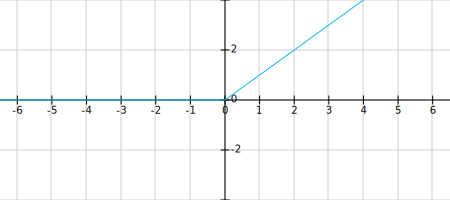
\includegraphics[width=0.6\linewidth]{imgs/02-Referential/02-ReLU.png}
            	\caption[Representación ecuación ReLU]{Representación ecuación ReLU.}
        	    \label{fig:ReLU}
            \end{figure}%
            
            La ecuación de ReLU equivale a decir que todos los valores negativos se reemplazaran por cero, en tanto que, los positivos mantendrán su valor original. Sus principales ventajas son: bajo coste computacional, por tanto ayuda a reducir el tiempo que puede llevar el entrenamiento, en comparación con otras funciones de activación. Converge más rápido. No tiene el problema de gradiente de fuga que sufren otras funciones de activación como sigmoide o tanh. 
            
            Por otro lado, para el calculo de la deriva de la función, requerida durante la etapa de entrenamiento de la red neuronal, basta con poner un condicional como se muestra en la ecuación \ref{EQ:ReLu_Derivada}.
            
            \begin{equation}
                \label{EQ:ReLu_Derivada}
                y' = 
                \begin{cases}
                  0, & \text{if}\ x< = 0 \\
                  1, & \text{para mayores a cero.}
                \end{cases}
            \end{equation}
            
            Puesto que ReLU es cero para todas las entradas negativas, es probable que alguna unidad no se active en absoluto lo que suele ser deseado en redes neuronales. Sin embargo, esta gran cualidad también puede ser su gran desventaja en algunos casos. Ya que puede llevar a la 'muerte' de las neuronas. Una neurona ReLU está 'muerta' si está atrapada en el lado negativo y siempre emite 0. Debido a que la pendiente de ReLU en el rango negativo también es 0, una vez que una neurona se vuelve negativa, es poco probable que se recupere. En tal caso, las neuronas dejan de tener un rol en la discriminación de la entrada y son esencialmente inútiles.

    \subsection{Funciones de pérdida}
        \label{sub:FrameLossFunction}
        
        La razón de entrenar modelos en inteligencia artificial es encontrar valores para los parámetros del modelo que representen más acertadamente el peso o impacto de cada uno dentro de de un conjunto de datos de entrenamiento, de forma que las predicciones estén cada vez más cercanas al valor esperado en la salida del sistema. En otras palabras reducir el error.
        
        Dicho lo anterior, y antes de poder reducir el error que tiene un modelo de inteligencia artificial es necesario calcular dicho error, para esto posible definir una función de pérdida $l(x)$ que mida que tan malos o lejanos son los valores obtenidos en una predicción de un modelo de inteligencia artificial. 
        
        Existen varias funciones de pérdida como el error cuadrático medio \index{MSE} o entropía cruzada\index{Entropía cruzada}, cada una con características particulares y, por tanto, su uso o selección puede depender de diversos factores como el tipo de algoritmo seleccionado o incluso la naturaleza de los datos de entrenamiento.
        
        \subsubsection{Error Absoluto Medio (MAE) / Pérdida L1\index{MAE}}
        \label{sub2:FrameMAE}
            
            Una forma simple de estimar el error entre los valores obtenidos y los esperados, consiste simplemente en la suma de los valores absolutos de la diferencia entre los valores obtenidos y los esperados. La ecuación \ref{EQ:MAE} muestra la expresión matemática de esté método.
            
            \begin{equation}
            	\label{EQ:MAE}
            	MAE = \frac{ \sum_{i=0}^{n} \left | y_i - y'_i \right |}{n}
            \end{equation}
            
            Siendo $y$ el vector de valores esperados durante el entrenamiento y $y'$ el vector equivalente obtenido.
            
        \subsubsection{Error cuadrático medio (MSE) / Pérdida L2\index{MSE}}
        \label{sub2:FrameMSE}
            
            El método de error cuadrático medio permite estimar el error entre los valores obtenidos y los esperados, a partir de la suma de los valores de la diferencia entre los valores obtenidos y los esperados elevada al cuadrado. Esto conlleva una penalización más marcada entre errores grandes en comparación con errores pequeños. La ecuación \ref{EQ:MSE} muestra la expresión matemática de esté método.
            
            \begin{equation}
            	\label{EQ:MSE}
            	MSE = \frac{ \sum_{i=0}^{n} (y_i - y'_i)^2}{n}
            \end{equation}
            
            Siendo $y$ el vector de valores esperados durante el entrenamiento y $y'$ el vector equivalente obtenido.
        
        \subsubsection{Entropía cruzada\index{Entropía cruzada}}
            \label{sub2:FrameCrossEntropy}
            
            El método de entropía cruzada aplicado a problemas de optimización combinatoria fue explorado por Rubinstein \cite{Rubinstein1997CrossEntropy}, aplicándolo inicialmente a redes estocásticas complejas y posteriormente en la estimación de la probabilidad de eventos raros. Se basa en el principio de máxima entropía propuesto por Jaynes \cite{Jaynes1957InformationTheory} y cuya exactitud fue demostrada por Shore y Johnson \cite{Shore1980}.
            
            La entropía cruzada puede utilizarse para medir la precisión de los valores pronosticados (el error), matemática (ver ecuación \ref{EQ:CE}) y conceptualmente se relaciona con la estimación por máxima verosimilitud. En otras palabras la suma negativa de la multiplicación de los valores del vector esperado por los logaritmos de los valores del vector de resultado.
            
            \begin{equation}
            	\label{EQ:CE}
            	CEL = - \sum_{i=0}^{n} y_i log(y'_i)
            \end{equation}
            
            Siendo $y$ el vector de valores esperados durante el entrenamiento y $y'$ el vector equivalente obtenido.
        
        \subsubsection{Pérdida de bisagra / Pérdida SVM\index{SVM}}
        \label{sub2:FrameSVM}
            La función de pérdida de bisagra (hinge loss en inglés), es usada en la clasificación de ``margen máximo'' en especial dentro de SVM\index{SVM}. Permite saber el grado de certeza de la predicción a partir de los mismos valores predichos. La ecuación \ref{EQ:SVMLoss} muestra la expresión matemática de esté método.
        
            \begin{equation}
            	\label{EQ:SVMLoss}
                \sum_{j \neq i}^{n} \max(0, y_j - y_i + 1)
            \end{equation}
            
            Siendo $y_j$ el valor obtenido en una de las posiciones del vector de resultados y $y_i$ el valor obtenido en cada una de las pociones del vector de resultados diferente de $y_j$.
        
        \subsubsection{Error de sesgo Medio (MBE) \index{MBE}}
        \label{sub2:FrameMBE}
        
            Aunque este método es quizá el menos común, en el campo de aprendizaje automático ya que su precisión es inferior a la de otros métodos, permite determinar si el modelo tiene un sesgo positivo o negativo. La ecuación \ref{EQ:MBE} muestra la expresión matemática de esté método.
            
            \begin{equation}
            	\label{EQ:MBE}
            	MBE = \frac{ \sum_{i=0}^{n} ( y_i - y'_i )}{n}
            \end{equation}
                
            Siendo $y$ el vector de valores esperados durante el entrenamiento y $y'$ el vector equivalente obtenido.
        
    \subsection{Descenso de gradiente}
    \label{sub:FrameGradient}
    
        Reducir el tamaño del error entre lo que predice un sistema de inteligencia artificial y el valor esperado es quizá la premisa más importante durante la etapa de entrenamiento. Aquí es importante entender qué es el tamaño del error y cómo se mide ese error. De forma general, el error en la predicción es la diferencia entre el valor esperado y el predicho por el sistema IA (vea la sección \ref{sub:FrameLossFunction} para profundizar en el concepto de funciones de pérdida). Entré más pequeño sea el tamaño del error, significa un mejor ajuste del sistema a los datos de entrenamiento (Ver sección \ref{Sec:FrameDataset} Referencia a creación de dataset para más detalle sobre conjuntos de datos), es decir una mejor caracterización de los datos. Es importante mencionar que un sobre ajuste en el entrenamiento puede ser problemático durante la ejecución con conjuntos de datos diferentes a los de entrenamiento, pero este tema es tratado en la sección \ref{sub:FrameOverfitting}.
        
        Durante el entrenamiento de una red neuronal artificial se utiliza el algoritmo de propagación hacia atrás o Back Propagation en inglés (El algoritmo de Back propagation\index{Back propagation} se explica en detalle en la sección \ref{sub:FrameBackPropagation}), este algoritmo debe calcular de forma iterativa los valores para cada neurona que minimicen el error general. Sin embargo, encontrar el valor mínimo para algunas funciones puede ser sencillo, como el caso presentado en la figura \ref{fig:X^2}, pero no todas las funciones tienen una forma tan clara para identificarlo, como el caso de la figura \ref{fig:SillaMontar}.
        
        \begin{figure}[ht!]
        	\centering
        	\includegraphics[width=0.6\linewidth]{imgs/02-Referential/02-X^2.png}
        	\caption[Gráfica de la función $f(x) = x^2$]{Gráfica de la función $f(x) = x^2$.}
    	    \label{fig:X^2}
        \end{figure}%
        
        \begin{figure}[ht!]
        	\centering
        	\includegraphics[width=0.6\linewidth]{imgs/02-Referential/02-X^2-Y^2.png}
        	\caption[Gráfica de la función $z={x}^{2}-{y}^{2}$]{Gráfica de la función $z={x}^{2}-{y}^{2}$.}
    	    \label{fig:SillaMontar}
        \end{figure}%
 
        Él mínimo de una función puede ser calculado de forma directa tomando su derivada e igualándola a cero. Sin embargo, eso solo es posible si la función tiene forma cerrada, lo cual no siempre es posible con las funciones de estimación de error en redes neuronales.
        
        Un segundo método consiste en ubicarse en cualquier punto de la función y avanzar de forma iterativa, buscando en cada paso estar en un punto inferior tratando de descender al punto más bajo. Para entender mejor considérese el siguiente ejercicio mental: Si una persona se encuentra en un punto no definido de una montaña, con los ojos vendados y debe encontrar la ruta que lo lleve a la parte baja de la montaña sin ver. En forma general la persona podrá moverse en cuatro direcciones (o 360 si desea comprobar la inclinación del terreno circundante cada grado de giro), cada vez que la persona identifique la dirección que le lleva más abajo respecto a las otras dará un paso, y este proceso lo repetirá de forma indefinida hasta que encuentre punto en el que todas las direcciones estén al mismo nivel. Este método es conocido como descenso de la colina o hill climbing.
        
        El principal inconveniente en la implementación del ejercicio mental expuesto, es que se debe realizar los cálculos para las cuatro direcciones antes de poder definir la dirección a avanzar, una forma de reducir esos costos computacionales consiste en el uso del gradiente. El gradiente es la generalización vectorial de la derivada, es decir, un vector con 'N' dimensiones y sobre el que se calcula para cada dimensión su derivada parcial, como muestra en la ecuación \ref{EQ:Gradient}, obteniendo de forma general la pendiente en un determinado punto. 
        
        \begin{equation}
            \label{EQ:Gradient}
            \nabla f=\left[\frac{\partial f}{\partial x_1}, \frac{\partial f}{\partial x_2}, \ldots \frac{\partial f}{\partial x_n} \right]
        \end{equation}
        
        Siendo $\nabla f_x$ el vector que contiene la información de cuanto crece la función en un punto especifico $x$ por cada dimensión de la función de forma independiente.
        
        A partir de la pendiente obtenida con uso del gradiente, es posible saber si un punto en una función sube o baja y, usando este mismo razonamiento, bastará con ir en contra de la pendiente en cada paso para encontrar cada vez un punto menor. Es justo aquí donde entra en juego el uso del algoritmo del descenso de gradiente en redes neuronales artificiales.
        
        El descenso de gradiente fue originalmente propuesto por Cauchy en 1847 \cite{Cauchy1847}, es un algoritmo de optimización iterativa, que se encarga de buscar el mínimo local yendo en contra de la pendiente dando pequeños pasos, usando información de la primera derivada y se ha convertido en uno de los pilares del aprendizaje automático, ya que durante la etapa de entrenamiento, permite reducir el valor del error entre la salida obtenida por la red y el valor esperado sin un excesivo costo computacional.
        
        Ahora bien, ir en contra de la derivada para definir la dirección de avance es solo una parte del razonamiento del descenso del gradiente, otro punto importantes es cuál debería ser la longitud del paso, es decir, qué tanto avanzar en cada paso para no pasar de largo y tener que regresar o inclusive nunca llegar. Para esto se agrega un parámetro $\alpha$ adicional llamado tasa de aprendizaje\index{Tasa de aprendizaje} o learning rate (ver sección \ref{sub2:LearningRate}, para mayor detalle sobre tasa de aprendizaje), como se muestra en la ecuación \ref{EQ:GradientDescendent}.

        \begin{equation}
            \label{EQ:GradientDescendent}
            -\alpha \nabla f
        \end{equation}
        
        Siendo $\alpha$ un valor pequeño, por ejemplo 0.3 y $\nabla f$ el vector del gradiente. Es importante considerar que $\alpha$ puede cambiar tras cada paso, y pueden existir varias criterios para ello, como incrementar su valor si el gradiente es grande y reducirlo en caso contrario, o simplemente ir reduciéndolo paulatinamente a medida que se realizan más iteraciones.
        
        Así pues, teniendo la dirección y el tamaño del paso a dar es posible calcular, dada una posición $x$ la siguiente posición $\hat{x}$.
        
        Finalmente, es necesario identificar si el algoritmo ha llegado a su fin, es decir, si se llegó al mínimo de la función. Una forma de hacerlo es calcular la diferencia entre $x$ y $\hat{x}$, si es menor que un umbral se puede dar por finalizado. También se puede simplemente realizar un número especifico de iteraciones.
        
        Una consideración especial, sin embargo, es que este tipo de métodos iterativos, no siempre permiten llegar de forma inexorable a un mínimo global de la función, sino más bien a mínimos locales, estos son puntos mínimos respecto a los valores a su alrededor como se muestra en la gráfica \ref{fig:LocalMin}. Aunque también cabe destacar que en el área del aprendizaje automático existen estrategias par intentar sortear los mínimos locales, como puede ser realizar varios entrenamientos con valores iniciales aleatorios e ir variando la tasa de aprendizaje.
 
        \begin{figure}[ht!]
        	\centering
        	\includegraphics[width=0.6\linewidth]{imgs/02-Referential/02-localmin.png}
        	\caption[Mínimos locales]{Mínimos locales. el punto a) corresponde a un mínimo local en la función, en tanto que b) corresponde al valor mínimo real de toda la función.}
    	    \label{fig:LocalMin}
        \end{figure}%
        
        \subsubsection{Tasa de aprendizaje\index{Tasa de aprendizaje}}
        \label{sub2:LearningRate}
            
            El concepto de tasa de aprendizaje\index{Tasa de aprendizaje} consiste en un hiper parámetro de las redes neuronales u otros modelos de aprendizaje supervisado, que permite definir que tan rápido aprende, en otros términos, que tan grande puede ser el cambio que se aplica a las variables de un modelo que se pretende ajustar.
            
            Las principales consideraciones de este parámetro radican en que si se asigna un valor muy pequeño, así mismo serán las actualizaciones a las variables del modelo, por lo que se requerirá de muchas iteraciones para que los cambios sean perceptibles, es decir aprenderá muy lentamente.
            
            Por otro lado, si la tasa de aprendizaje es muy alta, esto podría causar que las actualizaciones a las variables del modelo estén saltando de un lado al otro rodeando el error mínimo haciendo que, incluso, nunca se converja en una solución óptima.
            
            Ambos casos, una tasa muy alta o muy baja pueden llevar al problema de desvanecimiento o a la explosión del gradiente (ver sección \ref{sub2:GradientVanishing} para mayor detalle).
        
        \subsubsection{Explosión y desvanecimiento del gradiente}
        \label{sub2:GradientVanishing}
        
            De forma general el descenso del gradiente\index{Descenso del gradiente} permite calcular el cambio que debe hacerse en las variables de un modelo (pesos), realizando esto iterativamente este cambio (gradiente) va impactando en todo el modelo. Sin embargo, está misma iteración o llamado recursivo trae con sigo un problema y es llevar el gradiente a un extremo superior muy alto o a un extremo inferior muy pequeño, esto se conoce como explosión y el desvanecimiento del gradiente.
        
            La explosión y el desvanecimiento del gradiente (en inglés Exploding Gradients y Vanishing Gradients respectivamente) son un problema que afecta en especial a las redes muy profundas (con muchas capas) como el caso de las redes neuronales recurrentes\index{RNN} (ver \ref{sub:FrameRNN}).
            
            La explosión del gradiente ocurre cuando cuando en el modelo se genera una importancia exageradamente alta a los pesos, sin razón aparente, con lo que las entradas pierden importancia para el modelo. Aunque es un problema que no se puede predecir a priori es fácil de resolver con el truncamiento de los gradientes, evitando que sobrepasen un determinado umbral.
            
            Por otro lado, el desvanecimiento del gradiente o gradiente desvanecido ocurre cuando los cambios del gradiente son tan pequeños que el modelo deja sencillamente de aprender. Aunque es un es un problema mucho más difícil de resolver se han desarrollado mecanismos como de LSTM (ver sección \ref{fig:RNN-lstm}) para el caso de las redes recurrentes\index{RNN} o el uso de Redes Residuales\index{ResNet} para otro tipo de redes.
        
            La naturaleza de este problema está, como se mencionó, en la repetición de la operación y la constitución misma de la regla de la cadena usada por el algoritmo de propagación hacia atrás\index{Back propagation} (ver sección \ref{sub:FrameBackPropagation}). Supóngase una red de $t$ capas, cuando $t$ es un número grande, la operación iterativa aplicada a una función de activación\index{Función de activación} $f$ para obtener el gradiente, es decir la deriva de dicha función, sería como se muestra en la ecuación \ref{EQ:VanisingGradient}.
            
            \begin{equation}
                \label{EQ:VanisingGradient}
                {f'}_i(x) = \prod_{i=t-1}^{1} f_i(x) * {f'}_{i+1}(x)
            \end{equation}
            
            Es evidente que si al tener multiplicaciones sucesivas si se cae en un número grande éste se irá incrementando iterativamente y por otro lado los números pequeños se irán reduciendo sucesivamente. De aquí se identifica la importancia de la selección de la función de aprendizaje\index{Función de activación} más adecuada para cada problema.
            
    \subsection{Propagación hacia adelante (Forward propagation)}
    \label{sub:FrameForwardPropagation}
    
        En el campo de las redes neuronales artificiales\index{Redes neuronales} se les suele mencionar como un modelo inspirado en las las redes neuronales biológicas y, aunque dista mucho el entendimiento de las segundas permiten inferir el comportamiento esperado de las primeras.
        
        Una neurona biológica en forma general la componen tres partes: las dendritas, el cuerpo y los axones. Por medio de la sinapsis, la neurona recibe en las dendritas los mensajes de otras neuronas que la preceden, posteriormente en el cuerpo realiza la ``suma'' de todas las señales de excitación o inhibición, y si la señal de excitación es mayor transmite un un mensaje en forma de diferencia de potencial, a otras neuronas, usando su axón.
        
        En el campo de las redes neuronales artificiales es posible caracterizar a las neuronas por dos funciones: la función base (ver ecuación \ref{EQ:FuncionBase}) y la función de activación\index{Función de activación} (ver \ref{sub:FrameActivationFunctions}). Además, cada neurona está conectada a las neuronas de otras capas y asociado a cada conexión existen valores que determinan el efecto que tiene la neurona sobre las siguientes, esto se conoce como peso sináptico y se denomina como $w_{ij}$, siendo $w$ el efecto que la neurona $i$ sobre la neurona $j$ estando $i$ y $j$ en capas sucesivas.
        
        \begin{equation}
            \label{EQ:FuncionBase}
            u_i(w, x) = b + \sum_{j=0}^n w_{ij} * x_j 
        \end{equation}

        El algoritmo de propagación hacia adelante (Forward propagation en inglés) se utiliza para replicar el comportamiento de cada neurona biológica a lo largo de toda la red, esto es, ir transmitiendo las señales de las capas anteriores a las siguientes. Para esto el algoritmo toma las entradas a la neurona les aplica la función base (ecuación \ref{EQ:FuncionBase}), posteriormente, el resultado de la función base es pasado a la función de activación\index{Función de activación}. 
        
        De esta forma, los valores de entrada $x[...]$, sus pesos $w$ y el sesgo propio de la neurona $b$, generan una salida $y[...]$ que se convertirán en la entrada de las neuronas de la siguiente capa, repitiendo este proceso desde la primera hasta ultima capa de la red, como se muestra en la figura \ref{fig:PerceptronMulti2}.
        
        \begin{figure}[ht!]
        	\centering
        	\includegraphics[width=0.6\linewidth]{imgs/02-Referential/02-PerceptronMulticapa.png}
        	\caption[Modelo del Perceptrón multi capa]{Modelo del Perceptrón multi capa.}
    	    \label{fig:PerceptronMulti2}
        \end{figure}%
    
        El resultado de la capa final será la inferencia o predicción que es capaz de realizar un modelo para un conjunto de datos de entrada. Para que los resultados sean los esperados los pesos sinápticos $w$ y los sesgos $b$ deberán ser actualizados durante la etapa de entrenamiento y para ello se hace uso de los algoritmos de descenso de gradiente\index{Descenso de gradiente}(ver sección \ref{sub:FrameGradient}) y de propagación hacia atrás\index{Back propagation} (ver sección \ref{sub:FrameBackPropagation}).
        
    \subsection{Propagación hacia atrás (Back propagation)}
    \label{sub:FrameBackPropagation}
    
        Dentro del campo aprendizaje automático\index{Aprendizaje automático} se busca establecer las relaciones entre un conjunto de valores de entrada $x = [x_1, x_2, x_n$ y un conjunto de salida $y = [y_1, y2, y_m]$, en otras palabras que a partir de una entrada $x$ se pueda tener una salida conocida $y$. Para lograr esto se define un modelo que contemple las $n$ dimensiones de entrada de cada neurona para cada elemento de $y$, por ejemplo, es posible definir el modelo de la forma: $y=wx+b$.
        
        Dado que $x$ es un valor invariable es posible ajustar los valores de $w$ y de $b$ de forma que para cualquier valor $x$ de entrada se aproxime a los valores de salida $y$ correspondientes. El valor que debe ser ajustado se logra haciendo uso del algoritmo del descenso del gradiente\index{Descenso de gradiente}(ver sección \ref{sub:FrameGradient}), sin embargo es necesario que el ajuste de los parámetros del modelo se ajustes en cada neurona de la red.
    
        El algoritmo de propagación hacia atrás\index{Back propagation} o retropropagación (Back propagation en inglés) fue propuesto por Paul Werbos \cite{Werbos1975} en 1975 y representó un hito en el avance del desarrollo de las redes neuronales, pues fue el primero que permitió un entrenamiento eficaz, logrando que éstas realmente 'aprendieran' basados en la experiencia.
        
        La propagación hacia atrás es un método iterativo y recursivo que permite ir actualizando los 'pesos' de las neuronas, apoyándose en el descenso de gradiente y explota la conocida regla de la cadena.
    
        El proceso general de algoritmo de propagación hacia atrás\index{Back propagation} consiste en aplicar a todas las neuronas de la ultima capa (capa de salida) el algoritmo del descenso de gradiente, para identificar el cambio que debe hacerse en los pesos ($w$ y $b$). Una vez estimado el error en la ultima capa, dicho valor será multiplicado por el resultado de la aplicación de la derivada parcial a los pesos de las neuronas conectadas en la capa inmediatamente anterior.
        
        El proceso de ajustar los pesos, se realiza desde la última capa hasta llegar a la primera y se repetirá durante miles o millones de veces (dependiendo del problema) durante la etapa de entrenamiento, hasta que los pesos $w$ y $b$ de todas las neuronas y sus conexiones permitan que dada una entrada $x$ se obtenga una salida $y$ esperada, es decir, aprenda.
        
%    \subsection{HOG\index{HOG}}
%    \label{sub:FrameHOG}
%        \textcolor{red}{HOG}
%     
%    \subsection{K-means\index{K-means}}
%    \label{sub:FrameK-means}
%        \textcolor{red}{K-means}
%     
%    \subsection{Q-learnig\index{Q-learnig}}
%    \label{sub:FrameQ-learnig}
%        \textcolor{red}{Q-learnig}
%
%    \subsection{AdaBoost\index{AdaBoost}}
%    \label{sub:FrameAdaBoost}
%        \textcolor{red}{AdaBoost}

            
    \subsection{Función de clasificación Softmax}
    \label{sub:FrameSoftmax}
    \textcolor{red}{Softmax}
        
\section{Arquitectura de software}
\label{sec:FrameSwArchitecture}
        La arquitectura de software es la forma en que se describen los componentes de un sistema informático, las estructuras, los procesos que realizan y la manera en que interactúan, antes de la construcción del sistema. Por tanto es una tarea de diseño, desde el más alto nivel.
    
        Peter Freeman en \cite{Freeman1980}, define el diseño como ``\textit{una actividad que tiene que ver con la toma de decisiones importantes, con frecuencia de naturaleza estructural. Comparte con la programación el objetivo de abstraer una representación de la información y de las secuencias de procesamiento, pero en los extremos el grado de detalle es muy distinto}''.
        
        Por su parte Presman en \cite{Pressman2010}, define la arquitectura como ``\textit{Cuando se piensa en la arquitectura de una construcción, llegan a la mente muchos atributos distintos. En el nivel más sencillo, se considera la forma general de la estructura física. Pero, en realidad, la arquitectura es mucho más que eso. Es la manera en la que los distintos componentes del edificio se integran para formar un todo cohesivo. Es la forma en la que la construcción se adapta a su ambiente y se integra a los demás edificios en la vecindad. Es el grado en el que el edificio cumple con su propósito y en el que satisface las necesidades del propietario.}''. considerando además que es un a tarea de diseño agrega: ``\textit{La arquitectura no es el software operativo. Es una representación que permite 1) analizar la efectividad del diseño para cumplir los requerimientos establecidos, 2) considerar alternativas arquitectónicas en una etapa en la que hacer cambios al diseño todavía es relativamente fácil y 3) reducir los riesgos asociados con la construcción del software.}''

        La importancia de esta actividad radica entonces, en que en ella se plasman todas las decisiones importantes del sistema y como se mencionó la forma en que interactúan todas las partes involucradas en el mismo. De esta forma, y haciendo un símil con la construcción de edificios, de una correcta arquitectura puede depender, en gran medida, la estabilidad del sistema y, para el casos de sistemas informáticos la futura ampliación evitando la reconstrucción de partes importantes.
        
        Debido a su importancia, esta tarea suele ser ejecutada por personas experimentadas en el campo del desarrollo de software, usualmente conocidos como 'arquitectos de software'. Esta persona será la responsable de definir tanto las estructuras como mecanismos para la implementación de los diferentes artefactos del software. Para ello cuenta con la definición de soluciones generalizadas a problemas habituales, esto será explicado más adelante en la sección de patrones de desarrollo de software.
           
    \subsection{Patrón de desarrollo de software}
    \label{sub:FramePattern}
        El concepto de padrón se atribuye al arquitecto Christopher Alexander, quien en su publicación de 1977 \cite{Alexander1977}: ``\textit{Cada patrón describe un problema que ocurre una y otra vez en nuestro entorno, y luego describe el núcleo de la solución a ese problema, de tal manera que puede usar esta solución un millón de veces, sin hacerlo dos veces de la misma manera.}''.
        
        Prontamente, los especialistas en software se dieron cuenta que las ideas de Alexander, aun cuando estaban establecidas y orientadas hacia la construcción de edificios o similares, podrían ser extrapolables al desarrollo de software. Así Gamma et al. en su publicación de 1994 \cite{Gamma1994}, sentaron las bases en la definición de los patrones que permiten generalizar la mayoría de los problemas a los que se enfrenta un diseñador de software y brinda una orientación sobre como debería ser la correcta implementación.
    
    \subsection{Instancia única\index{Singleton} (Patrón)}
    \label{sub:FrameSingleton}
    
    ``\textit{Asegúrese de que una clase solo tenga una instancia y proporcione un punto de acceso global a ella.}'' \cite[Pág. 144]{Gamma1994}. (Traducción propia).
    
    Para algunos sistemas es de suma importancia que algunas clase solo tenga una única instancia, por ejemplo, para compartir información o recursos entre varios objetos o para que las modificaciones hechas por un objeto sea accesible de forma directa por otros. Un ejemplo de esto pueden ser el acceso a repositorios de datos como bases de datos o pilas de datos.
    
    Adicionalmente, debido a instancia única se puede aplicar un acceso controlado sobre la forma en que puede ser accedida y los requerimientos de acceso.
    
    \subsection{Método factoría (Patrón)}
    \label{sub:FrameFactoryMethod}
        
        ``\textit{Define una interfaz para crear un objeto, pero permita que las subclases decidan qué clase instanciar 'Método factoría' permite que una clase difiera la creación de instancias en subclases.}'' \cite[Pág. 121]{Gamma1994}. (Traducción propia).
        
        ``\textit{Los métodos de fábrica eliminan la necesidad de vincular clases específicas de la aplicación en el código. El código solo se ocupa de la interfaz de la clase; por lo tanto, puede funcionar con cualquier Clase definida por el usuario.}'' además, ``\textit{... El Método de Fábrica le da a las subclases un gancho para proporcionar una versión extendida de un objeto.}'' \cite[Pág. 123]{Gamma1994}. (Traducción propia).
        
        Con lo anterior es posible crear objetos de forma independiente para que las subclases puedan sobre escribir los métodos de la clase que heredan si fuera necesario.
        
    \subsection{Iterador (Patrón)}
    \label{sub:FrameIterator}
        ``\textit{Proporcione una forma de acceder a los elementos de un objeto agregado secuencialmente sin exponer su representación subyacente.}'' \cite[Pág. 289]{Gamma1994}. (Traducción propia).
        
        Gracias a este patrón es posible acceder a los elementos de un objeto agregado, como una lista,  sin exponer su estructura interna. 
        
    \subsection{Comando (Patrón)}
    \label{sub:FrameCommand}
        ``\textit{Encapsula una solicitud como un objeto, lo que te permite parametrizar clientes con diferentes solicitudes, solicitudes de cola o registro, y admite operaciones que no se pueden deshacer.}'' \cite[Pág. 263]{Gamma1994}. (Traducción propia).
        
        ``\textit{A veces es necesario emitir solicitudes a objetos sin saber nada sobre la operación que se solicita o el receptor de la solicitud. Por ejemplo, los kits de herramientas de la interfaz de usuario incluyen objetos como botones y menús que realizan una solicitud en respuesta a la entrada del usuario. Pero el juego de herramientas no puede implementar la solicitud explícitamente en el botón o menú, porque solo las aplicaciones que usan el juego de herramientas saben qué se debe hacer en cada objeto. Los diseñadores de kits de herramientas, no tienen forma de conocer al receptor de la solicitud o las operaciones que la llevarán a cabo.}'' \cite[Pág. 263]{Gamma1994}. (Traducción propia).
        
        Esto permite poner en cola y ejecutar solicitudes en diferentes momentos, lo que es además es útil para la interacción con pilas o con servicios que provean funcionalidades que no necesariamente impacten de forma directa en el cliente, ya que su naturaleza desacopla el objeto que hace la solicitud y la ejecución de la misma. 
        
        La naturaleza desacoplable brinda, además de lo mencionado, la flexibilidad de adicionar métodos o comandos, sin alterar el cliente y la forma en que éste interactúa, dando al sistema una capacidad mayor de escalabilidad.
    
    \subsection{Composición (Patrón)}
    \label{sub:FrameCompose}
        Consiste en la ``\textit{Composición de objetos en estructuras de árbol para representar jerarquías tanto de sus partes como de estructura completa. La composición permite a los clientes tratar objetos individuales y sus composiciones de objetos de manera uniforme.}'' \cite[Pág. 183]{Gamma1994}. (Traducción propia).
        
        ``\textit{El patrón compuesto define jerarquías de clase que consisten en objetos primitivos y objetos compuestos. Los objetos primitivos se pueden componer en objetos más complejos, que a su vez se pueden componer de otros, y así sucesivamente de forma recursiva.}'' \cite[Pág. 186]{Gamma1994}. (Traducción propia).
    
    \subsection{Método plantilla (Patrón)}
    \label{sub:FrameTemplateMethod}
        ``\textit{Consiste en definir el esqueleto de un algoritmo en una operación, aplazando algunos pasos a subclases. El Método de plantilla permite que las subclases redefinan ciertos pasos de un algoritmo sin cambiar la estructura del algoritmo.}'' \cite[Pág. 360]{Gamma1994}. (Traducción propia).
        
        Una de sus funciones es ``\textit{implementar las partes invariantes de un algoritmo una vez y dejarlo en manos de subclases para implementar el comportamiento que puede variar.}'' \cite[Pág. 361]{Gamma1994}. (Traducción propia).
        
        ``\textit{El método plantilla es una técnica fundamental para la reutilización de código. Tiene una gran importancia en las librerías de clases, porque son los medios para la generalización del comportamiento común en las clases de la biblioteca.}'' \cite[Pág. 362]{Gamma1994}. (Traducción propia).
        
        Este patrón suele combinarse con el patrón de método de factoría, pues la generalización que brinda una plantilla facilita la creación de objetos por parte de la factoría.
    
    \subsection{Pila de datos (Pool)}
    \label{sub:FramePool}
        ``\textit{Mejorar el rendimiento y el uso de la memoria reutilizando objetos de un grupo fijo en lugar de asignarlos y liberarlos individualmente.}'' \cite{Nystrom2014}. (Traducción propia).
        
        En  ciencias de la computación, una pila es un conjunto de objetos con características en común. El uso de pilas de datos u objetos es especialmente útil cuando se necesita el manejo y reuso de grandes cantidades de objetos, de esta forma, cuando cliente solicita un recurso a la pila este es entregado, sin embargo, cuando el cliente termina de usarlo, el recurso es mantenido en lugar de liberarse y perderse, lo cual mejora la eficiencia del sistema.
        
        A nivel de programación una pila es representado como un arreglo o una lista de un tipo de dato.
        
        Las permanencia de los datos en la lista dependerá del problema a tratar y, de igual forma la forma en que se almacenan o como se accede a cada elemento. Siendo posible almacenar y entregar los datos en la forma en que llegan, en forma inversa, o basado en características inherentes a los datos como el estado o un cualquier otro atributo.
        
    \subsection{Hilo}
    \label{sub:FrameThread}
        ``\textit{Un hilo es un flujo de control independiente dentro de un proceso, compuesto de un contexto (que incluye un conjunto de registros) y una secuencia de instrucciones para ejecutar. Por flujo de control independiente, nos referimos a una ruta de ejecución a través del programa.}'' \cite[Pág. 58]{Wadleigh2000}. (Traducción propia).
    
        Un hilo o subproceso en e campo de la computación es un el paquete de instrucciones procesamiento más pequeña que se puede realizar en un sistema operativo. Es el modelo de programación que permite que los procesos (o subprocesos) se ejecuten simultáneamente. Solo programa con capacidades de subprocesamiento múltiple permite que subprocesos individuales (o hilos) se ejecuten aparentemente al mismo tiempo.
        
        Una de las principales ventajas es que si un proceso se divide en múltiples subprocesos, y cada función de subproceso se considera como un trabajo, entonces aumenta el número de trabajos completados por unidad de tiempo, lo que aumenta el rendimiento del sistema.
    
    \subsection{Servicio REST}
    \label{sub:FrameService}
        En el campo de la arquitectura de software, el concepto de servicio hace referencia a una o varias piezas de software que permiten el acceso a diferentes recursos a través de una interfaz claramente establecida.
        
        REST (REpresentational State Transfer) es un modelo arquitectónico para desarrollar servicios web, descrito por Roy Fielding en el año 2000 \cite{Fielding2000}. Los servicios REST se basa en el estándar de transferencia de hipertexto (HTTP) y hace uso de los métodos que lo componen. En los últimos años ha ganado gran popularidad en el campo del desarrollo se sistemas de información, debido a su simplicidad y velocidad.
        
        ``\textit{Un servicio REST se define como una agregación de diferentes recursos a los que se puede acceder desde un URI base. Un recurso representa una entidad del mundo real cuyo estado está expuesto y se puede cambiar accediendo a un URI (identificador universal de recursos).}'' \cite{Pautasso2008}. (Traducción propia).
        
\section{Conjuntos de datos}
\label{Sec:FrameDataset}
    
    El conjunto de datos\index{Conjunto de datos} ('Data set' en inglés) es una agrupación de elementos con características similares de los cuales se desea que una Inteligencia Artificial\index{Inteligencia Artificial} reconozca las características intrínsecas a los elementos para, posteriormente, poder aplicar las inferencias aprendidas por el sistema a información nueva, sea esta, imágenes, textos, acciones o cualquier otro.
    
    Dentro del campo del aprendizaje automático, la creación de un conjunto de datos es en si misma una área de estudio, debido a la importancia fundamental de ellos. Sin datos no es posible hacer que un sistema ``aprenda''. A causa de esto, en cualquier proyecto de Inteligencia Artificial\index{Inteligencia Artificial} una de las actividades que demandan una gran cantidad de esfuerzo y tiempo es la preparación de un conjunto de datos.
    
    Cuando se prepara un conjunto de datos para entrenar una red neuronal\index{Redes neuronales}, es necesario contar con una cantidad suficientemente amplia para evitar o mitigar el sobre entrenamiento\index{Overfitting} (ver \ref{sub:FrameOverfitting}). Sin embargo, el tamaño no es la única consideración, la calidad de los datos es fundamental para contar con un buen Data set. 
    
    En muchas ocasiones para lograr la calidad de los datos es necesario realizar algunas etapas de preparación antes de que los sean aceptables para un entrenamiento. Considérese la figura \ref{fig:DatasetSteps} para establecer las etapas necesarias para la constitución de un Conjunto de datos\index{Conjunto de datos} para un sistema de aprendizaje automático\index{aprendizaje automático}.

    \begin{figure}[ht!]
    	\centering
    	\includegraphics[width=0.8\linewidth]{imgs/02-Referential/02-dataset-steps.png}
    	\caption[Pasos para la creación de conjuntos de datos.]{Pasos para la creación de conjuntos de datos.}
	    \label{fig:DatasetSteps}
    \end{figure}%
    
    Es importante mencionar que no todas las etapas son obligatorias, éstas dependerán de la calidad, la fuente y el formato originales de los datos.
    
    \subsection{Definición de los datos y fuentes necesarias}
        El primer paso en la preparación de un Data set consiste en definir qué se desea que el sistema aprenda, por ejemplo: identificar identificar evento anómalos en un entorno definido. A partir de esto es necesario establecer que posibles fuentes de información se tienen, por ejemplo: Imágenes, secuencias de vídeo, acelerómetros, o cualquier otro mecanismo del cual se puedan obtener los datos. 
        
        Junto con esto se identifica la estructura que tiene los datos en la fuente, por ejemplo: una matriz de píxeles, un flujo de números en el tiempo o cualquier otro, identificando completamente qué dato contiene cada variable obtenida de la fuente.
        
    \subsection{Recopilación de datos}
        La calidad y cantidad de los datos de entrenamiento puede marcar el éxito del entrenamiento. La recopilación de datos consiste en acumular datos de la mayor cantidad de fuentes posibles que cumplan con la definición hecha anteriormente. Una consideración fundamental en aprendizaje automático\index{Aprendizaje automático} es contar con una cantidad amplia de datos. Por eso, el proceso de recopilación de datos debe ser hecho de forma que se tenga un conjunto amplio, por ejemplo, para el análisis de imágenes usando redes convolucionales\index{CNN} se suelen considerar decenas de miles, cientos de miles o incluso millones de imágenes. De igual forma, si la información a utilizar como conjunto de entrenamiento depende del tiempo, es necesario contar con ventanas de tiempo suficientemente amplias que permita tener una muestra amplia.
        
    \subsection{Formateo de datos}
        Este paso busca hacer que todos los datos que recibirá el sistema para su entrenamiento sean consistentes en su estructura y en su valor, Por ejemplo, si una de las fuentes entrega un valor en dólares (USD\$1) y otra en euros (EUR\$1.00) es necesario definir un único formato y realizar la conversión a la moneda definida. O si se usan imágenes a escala de grises de un tamaño de 300x300 píxeles, es necesario llevarlas todas, sin importar la fuente, a escala de grises y al tamaño definido.
        
        Otro tipo de acción puede ser la \textbf{descomposición de los datos}, en caso de que la fuente genere datos complejos, éstos pueden ser descompuestos en partes más simples, por ejemplo: un valor de año mes día, puede ser separado en tres variables diferentes.
        
    \subsection{Limpieza y reducción de datos}
        En este paso se busca asegurar que toda la información a utilizar tiene aporte significativo durante el entrenamiento, para así, no aumentar excesivamente los recursos computacionales necesarios.
        
        Según lo mencionado, es beneficioso tener un conjunto amplio de datos, sin embargo, es necesario que asegurar que los datos tiene los atributos necesarios según lo definido, por ejemplo, si se busca identificar la postura de una persona en una imagen, puede ser de utilidad la eliminación de fotos donde haya más de una persona, pero también puede ser considerada la eliminación del fondo.
        
        En este paso, también se busca completar los datos, hasta donde sea posible, siguiendo con el caso de identificación de la postura de una persona en una imagen, puede ocurrir que no esté competa o al menos no tenga todos los puntos necesarios, en este caso en lugar de simplemente eliminarla podría ser aceptable completarla, esto es, proyectar extremidades ocluidas o cortadas de la foto usando las proporciones del cuerpo.
        
    \subsection{Normalización de datos}
        Un proceso normalización sobre los datos ayudan a asegurar la calidad de la información de forma que se reduzca el impacto negativo que pueden generar los valores anormales en el entrenamiento, un ejemplo de normalización de datos se demuestra en la ecuación \ref{EQ:MinMaxNormalization}.
        
        \begin{equation}
            \label{EQ:MinMaxNormalization}
            x_i^{'} = \frac{x_i - min(x)}{max(x) - min(x)}
        \end{equation}
        
        Donde $min$ representa el valor mínimo del conjunto $x$ y $max$ el mayor valor. De esta forma cada valor es ponderado respecto a su conjunto de pertenencia.
        
        Otra forma de normalización es 'discretizar' los datos. En algunos casos puede ser más eficiente trabajar con categorías discretas en lugar de valores continuos, por ejemplo, un sistema de recomendaciones basada en la edad podría tomar rangos de edades en lugar del valor de edad concreta.
        
    \subsection{Aumento de datos}
    \label{sub:FrameDataAugmented}
        
        La estrategia de aumento de datos es habitualmente utilizada cuando se dispone de muy pocos ejemplos para un entrenamiento \cite{Rojas2019heart}, ya que ayuda a reducir el sobre entrenamiento.
        
        ``\textit{La mejor manera de hacer que un modelo de aprendizaje automático se generalice mejor es entrenarlo en más datos. Por supuesto, en la práctica, la cantidad de datos que tenemos es limitada. Una forma de solucionar este problema es crear datos falsos y agregarlos al conjunto de entrenamiento.}'' \cite[Pag. 236]{Goodfellow2016}. (Traducción propia).
        
        El aumento de datos se logra aplicando diferentes transformaciones a los datos originales \cite{Fawzi2016DataAugmented}, por ejemplo, cuando se trata de imágenes es posible, a partir de una imagen original generar otras aplicando: rotaciones, cambio de escala, cambio de tonos, traslados entre otras. Gracias a esto se consigue una mejor generalización de los datos en la etapa de entrenamiento ya que las transformaciones no alteran la información intrínseca de los datos, pero aumentan la muestra, por ejemplo una imagen en espejo de un gato seguirá conteniendo un gato tanto en la original como en la transformada pero permitirá al sistema tener otro punto de vista del mismo objeto.
        
    \subsection{División del conjunto de datos\index{Data set}}
    \label{sub:FrameDatasetSplitting}
        Para saber que tan bueno es un sistema de aprendizaje automático\index{Aprendizaje automático} no basta con recopilar un conjunto amplio de datos, realizar el entrenamiento con todos ellos y estimar la precisión, de hecho esto es una mala practica debido a que no permite identificar un 'sobre entrenamiento' (ver \ref{sub:FrameOverfitting}) o sesgos que se podrán evidenciar posteriormente en la puesta en producción del sistema.
        
        La mejor opción para asegurar una tasa de precisión extrapolable a entornos fuera del conjunto de datos de entrenamiento; para sistemas de aprendizaje automático\index{Aprendizaje automático}, es dividir el conjunto en tres partes: Entrenamiento, Validación y Pruebas. La figura \ref{fig:DatasetSplitting} muestra dos momentos de división de los datos, en primer lugar una separación de los datos usados durante el tiempo de \textbf{entrenamiento} de los \textbf{datos de prueba}. Posteriormente una división adicional donde una parte de los datos de entrenamiento son tomados para \textbf{validación} y hacer los ajustes al modelo y verificaciones durante el proceso de entrenamiento. 
        
        \begin{figure}[ht!]
        	\centering
        	\includegraphics[width=0.8\linewidth]{imgs/02-Referential/02-dataset-splitting.png}
        	\caption[División del conjunto de datos.]{División del conjunto de datos.}
    	    \label{fig:DatasetSplitting}
        \end{figure}%
        
        
        \begin{itemize}
            \item \textbf{Subconjunto de entrenamiento}: Corresponde a los datos que serán usados para el entrenamiento del modelo.
            
            De este subconjunto dependerá lo que aprenda el sistema.
            
            \item \textbf{Subconjunto de validación}: Corresponde a los datos que serán usados durante la etapa de entrenamiento para refinar tanto el diseño del sistema como los parámetros.
            
            Este subconjunto ayudará a reducir el sobre entrenamiento del modelo durante la etapa de entrenamiento.
            
            \item \textbf{Subconjunto de pruebas}: Corresponde a los datos que serán usados para comprobar la precisión del modelo fuera de la etapa de entrenamiento, es decir, el que permitirá identificar que tan bueno es el modelo fuera del aprendizaje.
            
            La consideración más importante de este subconjunto es que los datos de éste nunca deben ser 'vistos' por el sistema durante la construcción y entrenamiento del sistema.
        \end{itemize}
        
        Aunque no existe un consenso sobre qué porcentaje debe ser asignado a cada parte, se suele dejar la mayor parte de los datos para el entrenamiento como tal, y es frecuente usar una distribución de 70-15-15 \cite{Valipour2016, Hemmat2015, Turabieh2019, Rojas2019heart}: 70\% para entrenamiento, 15\% para validación y 15\% para pruebas.
        
    \subsection{Sesgo de datos}
    \label{sub:FrameDatasetBias}
        El contar con un gran número de datos no es suficiente para decir que se cuenta con un buen conjunto de datos\index{Data set} para el entrenamiento, pues dentro de éstos puede existir un problema oculto conocido como ``Sesgo de datos''\index{Sesgo de datos}.
        
        ``\textit{Ningún sistema de inteligencia artificial tiene intencionalidad, pero las decisiones que aprende están basadas en los datos con los cuales ha sido entrenado, y si esos datos están sesgados (intencionadamente o no), el algoritmo decidirá sesgado, y ese sesgo puede tener consecuencias muy drásticas que afecten a la vida de las personas}'', Ramón López de Mántaras (Director del Instituto de Investigación en Inteligencia Artificial del Consejo Superior de Investigaciones Científicas (CSIC)) \cite{Vanguardia2017Sesgo}.
        
        El sesgo en los datos\index{Sesgo de datos} es una posibilidad de cualquier conjunto de datos, en mayor o menor medida, que se da en muchos casos de forma no intencional, por una limitada muestra, pero también puede ser dada por la fuente misma de los datos. El sesgo hace referencia al hecho de que los datos pueden contener características sobre los cuales se puede dar más importancia durante el entrenamiento de una Inteligencia Artificial y de las que el propio creador de la IA\index{Inteligencia Artificial} puede no tener conocimiento.
        
        El sesgo en los datos es un problema que impacta a los sistemas de aprendizaje automático\index{Aprendizaje automático} debido a la dependencia de los datos para el entrenamiento. Debido a esto, en los últimos años ha aparecido una creciente preocupación por el impacto de la Inteligencia Artificial en la vida diaria, no por el potencial mismo de esta tecnología, sino por los sesgos que este tipo de sistemas puedan tener \cite{Buolamwini2018Sesgo}. Sesgos como: decisiones injustificadamente influenciadas por la raza o el genero de la persona.
        
        Los sesgos se pueden presentar en cualquier conjunto de datos\index{Conjunto de datos}, sin importar su formato u origen, por ejemplo, se puede presentar cuando se construye un Data set para identificar rostros humanos en el cual la mayor cantidad de fotos corresponde a personas caucásicas de genero masculino y una escasa muestra de mujeres de origen africano. Este tipo de situaciones no necesariamente es intencional y pude deberse a la facilidad de conseguir los datos, en este caso imágenes, con las condiciones necesarias para el entrenamiento (fondo, iluminación, etc) de personas de regiones diferentes a la del investigador. También es habitual que cada pueblo haga herramientas para sus propias necesidades, así pues consciente o inconscientemente los creadores de este tipo de soluciones basadas en Inteligencia Artificial\index{Inteligencia Artificial} las construyen para sus contextos cercanos y, considerando que la mayor parte de investigaciones  y de empresas que trabajan en el desarrollo de estas tecnologías se encuentran en el norte de América, Europa y Asia, es entendible que inicialmente sus propios Data set estén sesgados a las características dominantes de su población.
        
        Otro sesgo que encontrado en los datos, que si bien al mirar hacia atrás pudo ser previsible, solo se notó su impacto bajo la mirada moderna de equidad, fue el presentado por Bolukbasi et al. \cite{Bolukbasi2016Sesgo} cuando se usa al modelo Word2Vec construido por investigadores de la empresa Google. Word2Vec es un modelo entrenado usando un corpus muy extenso de textos para inferir, entre otras cosas, la cercanía contextual entre palabras, de forma que la relación entre gato y animal es mayor que entre gato y televisor \cite{Mikolov2013Word2Vec}. Bolukbasi et al utilizaron Word2Vec para construir un sistema de analogías de forma que el sistema completara la palabra faltante, lo que mostraron Bolukbasi et al. es un sesgo de genero con el ejemplo: "Hombre es a programador como mujer es a X" donde la "X" fue reemplazada por "ama de casa" \cite{Bolukbasi2016Sesgo}. 
        
        Para cualquier investigador es evidente que el sesgo existente en Word2Vec no es causado intencionalmente por los investigadores de Google, sino que es un sesgo existente en la misma sociedad generadora de los textos, y como se menciono anteriormente es entendible el origen de estos sesgos, sin embargo, el ser entendible no significa que sea aceptable, pues aunque los sesgos como decidir enviar a prisión a una persona, por variables diferentes a su comportamiento, que unos sistemas funcionen mejor en función de su raza o que el genero defina las actividades de una persona pueden no ser socialmente aceptables.
        
        Aunque los sesgos mostrados pueden ser los de mayor impacto social en la actualidad, el sesgo de los datos afecta de forma negativa a cualquier sistema de aprendizaje automático, puede un sistema de IA entrenado para que reconozca una determinada enfermedad entrenarla con, por ejemplo, imágenes de mujeres con dicha enfermedad, llegar a inferir que los hombres no la padecen. O si se entrena a un asistente virtual para reconocer comandos de voz con un conjunto de datos constituido solo por archivos de audio de personas de España, podría tener una tasa de error muy alto cuando lo use una persona de origen americano, aun cuando se use el mismo idioma, pues la IA puede desarrollar un sesgo por la forma de pronunciar las palabras.
        
        \begin{figure}[ht!]
        	\centering
        	\includegraphics[width=0.8\linewidth]{imgs/02-Referential/02-dataset-no-bias.png}
        	\caption[Conjunto de datos sin sesgo.]{Conjunto de datos sin sesgo. Imagen tomada de \cite{Buolamwini2018Sesgo} donde se presenta una distribución bien balanceada entre rostros de personas de diferentes colores de piel y genero.}
    	    \label{fig:DatasetNoBias}
        \end{figure}%
        
        Para reducir el impacto del sesgo de datos es necesario no solo un conjunto de datos más amplio sino también más heterogéneo en su muestra, como el caso del proyecto {http://gendershades.org/} liderado por Buolamwini y Gebru \cite{Buolamwini2018Sesgo} donde muestran un conjunto más balanceado entre razas, colores de piel y géneros (ver figura \ref{fig:DatasetNoBias}), de forma que el sistema entrenado no tenga ninguna inclinación especial e injustificada por ninguna de las características fenotípicas y su aprendizaje esté mejor orientado a las características que se desean en la identificación de rostros.
        
    %Sitios de datos abiertos:
    %https://www.openml.org/
    %https://www.kaggle.com/
    
    
    \subsection{ImageNet (Data set)}
    \label{sub:FrameImageNet}
    
        El data set\index{Conjunto de datos} ImageNet es un conjunto compuesto por más de 14 millones de imágenes de alta resolución publicado y compartido en el año 2009 \cite{ImageNet2009}, creado por Deng et al.
        
        ``\textit{ImageNet es un conjunto de datos de imágenes organizado de acuerdo con la jerarquía de WordNet. Cada concepto significativo en WordNet, posiblemente descrito por múltiples palabras o frases de palabras, se denomina conjunto de sinónimos o synsets. Hay más de 100,000 synsets en WordNet, la mayoría de ellos son sustantivos (80,000+). En ImageNet, nuestro objetivo es proporcionar un promedio de 1000 imágenes para ilustrar cada synset. Las imágenes de cada concepto tienen control de calidad y anotación humana.}'' \cite{Imagenet2020Home} (Traducción propia).
        
        El conjunto Imagenet más que un repositorio de imágenes provee un listado de URLs de Internet donde se localizan las imágenes. Adicionalmente, para cada imagen se etiqueto diferentes objetos en ellas, hasta un total de 20 mil en todo el conjunto, donde se pueden encontrar etiquetas para: Aviones, gatos, espejos de coches, entre muchos otros.
        
        \subsubsection{Competencia para el reconocimiento visual}
        
        Adicional al data set y en apoyado en éste se creó el ``ImageNet Large Scale Visual Recognition Challenge [ILSVRC]'' \cite{Imagenet-ILSVRC15}, una competición para impulsar el desarrollo de las tecnologías en el campo de la identificación de objetos. Gracias a esto se han desarrollado modelos de identificación de objetos como "Inception V3" \cite{InceptionV32016}, creado y compartido por la empresa Google.
        
    \subsection{COCO (Data set)}
    \label{sub:FrameCOCO}
    
        Objetos comunes en contexto (En inglés Common Objects in Context - COCO) es un data set con una gran cantidad de imágenes (más de 300 mil) \cite{COCO2014} que cuenta con información detallada de los objetos comunes en ellas, de forma que puede ser usado para el entrenamiento de modelos para detección, segmentación o etiquetado de objetos. Los objetos fueron etiquetados utilizando segmentaciones por instancia para ayudar en la localización precisa de objetos. Dentro de sus características principales se encuentran:
        
        \begin{itemize}
            \item Más de 200 mil imágenes etiquetadas.
            \item 2.5 millones de instancias de objetos segmentados en todo el conjunto.
            \item 80 tipos de categorías de objetos.
            \item 250 mil imágenes de personas con puntos clave (articulaciones principales, cabeza, entre otras que permiten formar un esqueleto) marcadas.
        \end{itemize}
        
        \subsubsection{Competencia COCO para generación de esqueletos de personas en imágenes}
        \label{sub2:FrameCOCOKeyPoints}
        
            A partir de las 250 mil imágenes de personas y los 1.7 millones de puntos clave, se creó una competencia (``COCO Keypoints        Challenge'' \cite{Coco2020KeyPointsHome}) para impulsar el desarrollo de investigaciones de métodos que permitan la localización de personas y la generación de un esqueleto caracterice la postura de las personas. Como se muestra en la figura \ref{fig:COCOKeyPointChallenge}, este data set contiene puntos etiquetados para las articulaciones principales, el cuello y el centro de la cabeza en imágenes una o más personas en situaciones y posturas cotidianas.
        
            \begin{figure}[ht!]
            	\centering
            	\includegraphics[width=0.8\linewidth]{imgs/02-Referential/02-coco-keypoints.png}
            	\caption[Ejemplo de imágenes del COCO keypoint Challenge]{Ejemplo de imágenes del COCO keypoint Challenge \cite{Coco2020KeyPointsHome}.}
        	    \label{fig:COCOKeyPointChallenge}
            \end{figure}%

    \subsection{MPII Human Pose (Data set)}
    \label{sub:FrameMPII}
        
        Para impulsar la investigación en la estimación de la postura humana en imágenes en el año 2014, Andriluka et al. presentaron el conjunto de datos ``MPII Human Pose'' \cite{MPII2014}\index{Conjunto de datos}.
        
        Este conjunto de datos está compuesto por más de 25 mil imágenes y dentro del conjunto más de 40 mil personas con las articulaciones principales etiquetadas. El conjunto también tiene etiquetas para partes del cuerpo ocluidas y la orientación de la cabeza.
        
        El data set\index{Conjunto de datos} fue construido a partir de vídeos de Youtube, considerando varios frames, los cuales cuentan también con un marcado de orden de secuencia de cada uno. El conjunto de datos agrupa un total de 410 actividades diferentes, organizadas como se muestra en la figura \ref{fig:MPII}.
        
        \begin{figure}[ht!]
        	\centering
        	\includegraphics[width=0.8\linewidth]{imgs/02-Referential/02-MPII.png}
        	\caption[MPII Human Pose]{MPII Human Pose \cite{MPII2014}.}
    	    \label{fig:MPII}
        \end{figure}%
    
    \subsection{HumanEva (Data set)}
    \label{sub:FrameHumanEva}
    
        HumanEva es un data set\index{Conjunto de datos} de imágenes de actividades humanas hechas en laboratorio \cite{Sigal2010Humaneva, Humaneva2020Home}, es decir, fueron capturadas en un ambiente controlado (objetos e iluminación). Para la captura se utilizaron siete cámaras sincronizadas, cuatro de escala de grises y tres de color, de forma que el conjunto de datos contiene la información 3d de las personas filmadas.
        
        El conjunto de datos\index{conjunto de datos} se realizó con la participación de cuatro actores mientras realizaban diferentes actividades comunes (caminar, trotar, lanzar y atrapar una pelota, boxeo y algunas combinaciones). En total 40 mil fotogramas sincronizados.
        
    \subsection{FLIC (Data set)}
    \label{sub:FrameFLIC}
        
        FLIC es un conjunto de imágenes (con alrededor de cinco mil imágenes), generado a partir de 30 películas populares de cine de Hollywood \cite{FLIC2013}. El data set\index{Conjunto de datos} tiene diez etiquetas para las articulaciones superiores de las personas en las imágenes.
    
    \subsection{DMLSmartActions (Data set)}
    \label{sub:FrameDMLSmartActions}
    \textcolor{red}{DMLSmartActions}
    DMLSmartActions dataset: Dataset for human actions in smart
environments, (Jan. 2019), University of British Colombia, [Online].
Available: http://dml.ece.ubc.ca/data/smartaction/.
        
        
        UCF101: A Dataset of 101 Human Actions Classes From Videos in The Wild
        
        
        SBU Kinect Interaction Dataset SBU Kinect Interaction
Dataset is created by Yun and Honorio et al. [38] using Microsoft
Kinect for two-person interactions. There are 8 categories including 7 participants and 21 groups of interactive actions. The dataset contains 282 skeletal sequences and 6822 frames and 15 joints. https://ieeexplore.ieee.org/document/6239234
        
        
\section{Software y librerías}
\label{Sec:FrameSoftware}

    \subsection{Python}
    \label{sub:FramePython}
        ``Python es un lenguaje de programación interpretado, orientado a objetos y de alto nivel con semántica dinámica...'', ``...Python admite módulos y paquetes, lo que fomenta la modularidad del programa y la reutilización de código. El intérprete de Python y la extensa biblioteca estándar están disponibles en formato fuente o binario sin cargo para todas las plataformas principales, y se pueden distribuir libremente.'' \cite{Python2019}.
        
        Debido a flexibilidad, además de propiciar la facilidad en la legibilidad en el código, Python se ha convertido en el principal lenguaje utilizado en el desarrollo de librerías de índole científico en general y de inteligencia artificial en particular.
    
    \subsection{JSon}
    \label{sub:FrameJSon}
        ``JSON (JavaScript Object Notation) es un formato ligero de intercambio de datos. Es fácil para los humanos leer y escribir. Es fácil para las máquinas analizar y generar. Se basa en un subconjunto del lenguaje de programación JavaScript Standard ECMA-262 3rd Edition - December 1999. JSON es un formato de texto que es completamente independiente del lenguaje pero utiliza convenciones que son familiares para los programadores de la familia de lenguajes C, incluido C, C ++, C\#, Java, JavaScript, Perl, Python y muchos otros. Estas propiedades hacen que JSON sea un lenguaje ideal para el intercambio de datos.'' \cite{Json2019}.
    
    \subsection{Yaml}
    \label{sub:FrameYaml}
        Yaml es un lenguaje de serialización de datos basado en Unicode, pensado para que sea de fácil interpretación por humanos. Está diseñado para representar los principales tipos de datos de los lenguajes de programación ágiles. debido a su naturaleza como archivo plano puede ser usado por cualquier lenguaje de programación y presta especial utilidad para el envío de mensajes por Internet o para archivos de configuración \cite{Yaml2019}.
        
    \subsection{Tensorflow}
    \label{sub:FrameTensorflow}
        ``TensorFlow es una plataforma de código abierto de extremo a extremo para el aprendizaje de máquina (ML). Cuenta con un ecosistema integral y flexible de herramientas, bibliotecas y recursos de la comunidad que permite a los investigadores impulsar el estado del arte en ML y los desarrolladores pueden construir y desplegar fácilmente aplicaciones potenciadas por ML.'' \cite{GoogleTF2019}.

        TensorFlow fue desarrollado originalmente por el equipo de Google Brain Team, dentro del departamento de investigación de Machine Intelligence, con el propósito de llevar a cabo el aprendizaje automático y la investigación de redes neuronales profundas. Desde su lanzamiento como software de código abrieto, a finales del 2015, se ha convertido en una de la principales herramientas en la construcción de sistemas de inteligencia artificial.
        
    \subsection{Keras}
    \label{sub:FrameKeras}
        ``Keras es una API de redes neuronales de alto nivel, escrita en Python y capaz de ejecutarse sobre TensorFlow, CNTK o Theano. Fue desarrollado con un enfoque en permitir la experimentación rápida. Poder pasar de la idea al resultado con el menor retraso posible es clave para hacer una buena investigación.''
        
        Keras permite la creación fácil y rápida de redes neuronales, incluyendo convolucionales y redes recurrentes, así como combinaciones de las dos y, además, su ejecución en GPU. Aunque Keras no se encarga de las funciones matemáticas involucradas en el entrenamiento y aprendizaje de las redes neuronales, su popularidad radica en que expone una capa que simplifica el uso de las librerías matemáticas como Tensofflow.
        
        El desarrollo de Keras está respaldado principalmente por Google, y la API de Keras viene empaquetada en TensorFlow como tf.keras. Además, Microsoft mantiene el backend CNTK Keras. Amazon AWS mantiene la bifurcación Keras con soporte MXNet. Otras compañías contribuyentes incluyen NVIDIA, Uber y Apple (con CoreML).
        
    \subsection{Flask}
    \label{sub:FrameFlask}
        Flask es una librería escrita en lenguaje Python, que permite de forma rápida la creación y exposición de servicios REST \cite{Flask2019}.
        
    \subsection{Logging}
    \label{sub:FrameLogging}
        Una de las tareas más habituales en cualquier proyecto de software es el registro de los eventos que ocurren durante su ejecución. Normalmente se registran mensajes de errores o excepciones, pero también pueden ser almacenados mensajes como inicio de servicios u otros.
        
        Dentro de la funcionalidades incluidas en el ambiente Python, existe la librería 'Loggin'. ``Este módulo define funciones y clases que implementan un sistema flexible de registro de eventos para aplicaciones y bibliotecas. El beneficio clave de tener la API de registro proporcionada por un módulo de biblioteca estándar es que todos los módulos de Python pueden participar en el registro, por lo que el registro de su aplicación puede incluir sus propios mensajes integrados con mensajes de módulos de terceros.'' \cite{Logging2019}.
    
    \subsection{Microsoft Kinect}
    \label{sub:FrameKinect}
        Kinect es un dispositivo desarrollado por Microsoft, que estuvo en el mercado desde el año 2010 y fue descontinuado en el año 2017. Kinect es una barra horizontal diseñado para ser colocado longitudinalmente por encima o por debajo de la pantalla de vídeo (Ver fig. \ref{fig:Kinect}).
        
        \begin{figure}[ht!]
        	\centering
        	\includegraphics[width=0.8\linewidth]{imgs/02-Referential/02-Kinect.png}
        	\caption[Microsoft Kinect]{Microsoft Kinect.}
    	    \label{fig:Kinect}
        \end{figure}%

        El dispositivo cuenta con una cámara RGB, un sensor de profundidad, un micrófono de múltiples matrices y un procesador personalizado que ejecuta el software patentado, que proporciona captura de movimiento de todo el cuerpo en 3D reconocimiento facial y capacidades de reconocimiento de voz.

        Algunas de sus características más relevantes son: Iluminación infrarroja independiente (30 fps), Esqueleto de 25 puntos para un total de seis personas (cada persona tiene 25 articulaciones esqueléticas)
        Seguimiento del pulgar, seguimiento del final de la mano, gestos con las manos abiertas y cerradas. Alcance de operación de desde 0.5 metros cerca a 4.5 metros lejos \cite{Kinect2019}.

    \subsection{Web Sockets}
    \label{sub:WebSockets}

        ``WebSockets es una tecnología avanzada que hace posible abrir una sesión de comunicación interactiva entre el navegador del usuario y un servidor. Con esta  API, puede enviar mensajes a un servidor y  recibir  respuestas controladas por eventos sin tener que consultar al servidor para una respuesta.'' \cite{WebSockets2020}.

\section{Antecedentes}
\label{Sec:FrameRelatedWork}

    \subsection{Detección de objetos en imágenes}
    \label{sub:FrameObjectDetection}
        ``La detección de objetos es una tarea importante de visión por computadora que se ocupa de detectar instancias de objetos visuales de una determinada clase (como humanos, animales o automóviles) en imágenes digitales... '', para dar respuesta a ``... ¿Qué objetos están y dónde están?'' \cite{zou2019}. (Traducción propia).
    
        Durante las últimas dos décadas ha habido un amplio interés en el desarrollo de técnicas que permitan identificar objetos en imágenes. Aunque, las investigaciones en este campo se remontan más atrás, con trabajos como el presentado por Vaillant et al. haciendo uso de redes neuronales \cite{Vaillant1994} o pocos años más tarde LeCunn et al. presentando el uso de capas convolucionales, dentro de las redes neuronales tradicionales \cite{LeCun1998}. Aunque el uso de capas de convolución fueron muy limitadas en su momento,  debido a los requerimientos de computo, hoy en día que se han convertido en pieza fundamental de los desarrollos más resientes en el la visión por computador.
        
        Las propuestas para identificar objetos en imágenes pueden ser divididas en dos grupos, el primero está compuesto por los métodos que podrían llamarse tradicionales vigentes hasta el año 2014. Por otro lado, están los métodos basados en redes neuronales, los cuales mostraron su amplia superioridad respecto a los anteriores, destacando en el año 2014 el método denominado R-CNN \cite{Girshick2014} que logró una precisión de 58.5\% en conjunto de prueba ``The Pascal Visual Object Classes (VOC\index{VOC}) challenge''\cite{VOC2010}.
        
        \subsubsection{Métodos tradicionales}
        \label{Sub2:FrameObjectDetectionTraditional}
            Uno de los métodos de mayor popularidad, en detección de objetos, a principios de los años 2000 fue presentado por P. Viola y M. Jones \cite{Viola2001, Viola2004}, cuyo algoritmo, actualmente conocido como ``VJ Detector'' permitió la detección de rostros en tiempo real (15 cuadros por segundo) en una máquina con un procesador de 700MHz. 
            
            Según los propios autores, Viola y Jones, resaltan tres etapas y contribuciones clave de su trabajo. En primer lugar la representación integral de la imagen (Integral Image), que permite identificar rápidamente las características utilizadas por el detector. El segundo es un clasificador basado en AdaBoost \index{AdaBoost} que a su vez permite la selección de unas pocas características críticas. Finalmente, la combinación en cascada de clasificadores, lo que permitió descartar rápidamente zonas como el fondo, dando mayor tiempo de computo a las zonas prometedoras.
            
            En el año 2005, N. Dalal y B. Triggs, presentaron el método para la extracción de características conocido como ``Histograma de gradientes orientados'' (HOG\index{HOG} - Histogram of Oriented Gradients) \cite{Dalal2005}. El método de Dalal y Triggs se motivó en el problema de detección del peatón, y fue uno de los principales métodos para resolver este problema en su época.
            
            Dalal y Triggs propusieron una forma en la cual generalizar las características de una imagen a partir de la variación de luminosidad de cada píxel o conjunto de píxeles, en otras palabras, la generación de flechas que indican la dirección en la que los vecinos de un píxel son más oscuros respecto el píxel observado. Posteriormente, esas flechas son pasadas a un clasificador SVM\index{SVM} previamente entrenado que se encarga de identificar qué grupo de flechas se asemejan al conjunto extraído durante el entrenamiento.
            
            Basado en el método de HOG\index{HOG}, hacia 2008 Felzenszwalb et al. presentaron un modelo deformable basado en las partes (DPM\index{DPM} - Deformable Part-based Model) de los objetos que componen. Convirtiéndose en el método con mejores resultados hasta antes de la aparición de los métodos basados en Deep learnig. La estrategia de este método consistió en identificar las partes que componen un objeto, por ejemplo, en una persona, de igual forma que HOG\index{HOG}, se identifica el rostro, los brazos, las piernas, etc. por separado, para posteriormente otorgar una etiqueta de conjunto. Este método tubo gran éxito y fue mejorando hasta llegar a la versión 5 del mismo, en el año 2014, año en que fue superado ampliamente por los métodos basados en redes neuronales.
            
        \subsubsection{Métodos basados en deep learning}
        \label{Sub2:FrameObjectDetectionNN}
            En el año 2014 Girshick et al. presentaron R-CNN \cite{Girshick2014}, el resurgimiento de las redes convolucionales como mecanismo para el procesamiento de imágenes. RCNN consiste en dos etapas o estados, en primer lugar extrae cajas candidatas a objetos, luego cada una del cajas tomadas de la imagen original es escalada para ajustarla al tamaño de entrada de una red neuronal convolucional que previamente se entreno con el conjunto de datos de ImageNet \cite{ImageNet2009}, al finalizar el proceso un clasificador SVM\index{SVM} discriminaba si un objeto especifico se encontraba en la imagen procesada. La superioridad de este tipo de métodos se demostró con el conjunto de prueba del ``PASCAL VOC Challenge'' \cite{VOC2010} donde superó a los mejores métodos hasta entonces, con hasta un 25\% más de precisión.
            
            Aunque una mejora significativa en la precisión, RCNN presentaba un gran inconveniente para su implementación en dispositivos de bajo poder de computo, debido a los tiempos de procesamiento empleados, pues se generaba un gran número de cajas a procesar. El siguiente año a la presentación de RCNN, He et al. presentaron un método denominado SPP-Net que reduce el tiempo de procesamiento entre 24 y 101 veces \cite{He2015}. Este método tiene la ventaja de que evita la repetición del procesamiento de las características de convolución, ya que calcula los mapas de características de la imagen completa solo una vez, adicionalmente, los detectores son entrenados sobre regiones arbitrarías de longitud fija.
            
            El mismo 2015, nuevamente Girshick presentó Fast R-CNN \cite{Girshick2015}, una mejor a su propuesta inicial. Fast R-CNN logra que el tiempo de entrenamiento de la red VGG16\index{VGG}\cite{Simonyan2014VGG} sea 9 veces más rápida en comparación con R-CNN y hasta 213 veces más rápida en tiempo de prueba.
            
            Los trabajos de SPP-Net y Fast R-CNN, expusieron como principal problema de R-CNN en términos de rendimiento, la sobrecarga en la estimación de las regiones propuestas. En 2015 Ren et al. presentaron ``Faster R-CNN'', una red de propuesta de región (RPN\index{RPN}) que comparte características convolucionales con la red de detección, permitiendo así propuestas de región casi sin costo \cite{Ren2015}.
            
            Hasta este momento, los métodos expuestos para la detección de objetos estaban basados en dos estados: en un primer momento se genera un conjunto de regiones candidatas, a partir de búsquedas selectivas como ``Deep Mask'' \cite{Pinheiro2015}, RPN \cite{Ren2015} o ``Edge boxes'' \cite{Zitnick2014}. Posteriormente, las regiones de interés (RoI\index{RoI}) son pasadas por una red convolucional para determinar la pertenencia a una determinada clase. Si bien esta estrategia obtenía buenos resultados, seguía requiriendo alta carga de procesamiento. 
            
            Como respuesta y solución a los problemas de velocidad de los métodos de dos estados surgen los métodos de un estado. En el año 2016 Redmon et al. presentaron YOLO \cite{Redmon2016} (You Only Look Once), un cambio significativo respecto a los métodos anteriores, aunque con resultados similares en su precisión, logra el procesamiento de 45 cuadros por segundo, lo que permite su implementación en sistemas que requieran procesamiento en tiempo real. Pero incluso una velocidad aun mayor, 155 cuadros por segundo en una versión reducida de su diseño, aunque con menor tasa de éxito. La filosofía del modelo propuesto en YOLO, consiste en la integración en una única red la detección de los cuadros que delimitan un objeto y los porcentajes de probabilidad de pertenencia a una determinada clase, lo que permitió a los autores optimizar significativamente la cantidad de procesamiento requerida.
            
            También en 2016, Liu et al. presentaron SSD \cite{Liu2016}, el segundo detector de un solo estado. SSD Parte de la red VGG\index{VGG}\cite{Simonyan2014VGG} tradicionalmente utilizada para la clasificación de imágenes, pero elimina las capas de clasificación y agrega otras capas de convolución propias, logrando con un 74\% superar la precisión de YOLO de 63\% en el conjunto de prueba ``Pascal VOC'' \cite{VOC2010}.
            
            En 2017 Lin et al. presentaron una propuesta que denominan pérdida focal (focal loss) \cite{Lin2017} donde argumentan que la razón central del desequilibro entre ambas clases se debe a que hay una descompensación entre lo que son los objetos a detectar y el fondo de la imagen, en otras palabras que durante el entrenamiento, las regiones identificadas como fondo, por su cantidad, pueden abrumar los escasos ejemplos positivos, por tanto, proponen modificar el método de estimación de perdida de entropía cruzada, disminuyendo la perdida que se da a los casos bien identificados, logrando tasas de éxito y de velocidad comparables a los mejores métodos de su momento, como demostración de lo propuesto, los autores crearon un detector simple llamado RetinaNet \cite{Lin2017}.
            
            En 2018 Zhang et al. presentaron RefinaDet \cite{Zhang2018} con el objetivo de  integrar, aún más, la precisión de los modelos de dos etapas como R-CNN \cite{Girshick2014} y la velocidad de los modelos de una etapa como SSD \cite{Liu2016}. RefinaDet consiste en dos módulos interdependientes, donde el primero va eliminando los candidatos negativos, mientras que el otro módulo va realizando la clasificación sobre los restantes.

    \subsection{Localización de personas en una imagen}
    \label{sub:FramePersonDetection}
        La localización de una persona en una imagen consiste en separar la persona de todos los demás elementos de una imagen, sin importar la postura, la forma, el color o incluso la vestimenta que use. 
        
        Tener cada persona que aparece en una imagen claramente diferenciada, facilita la realización de tareas de índole superior, como identificar una postura o incluso una emoción, ya que permite centrar el análisis en los píxeles que conforman la persona, lo que reduce la cantidad de datos a analizar. 
        
        Una técnica comúnmente utilizada en el cine, la televisión y fotografía, conocida como croma o uso de croma, permite la extracción de la persona usando un fondo de un color homogéneo, usualmente verde, como se muestra en la figura \ref{fig:croma}. Sin embargo, esta técnica no puede ser aplicada de forma general, pues requiere de un ambiente controlado donde, además del fondo uniforme se controle la iluminación.
        
        \begin{figure}[ht!]
        	\centering
        	\includegraphics[width=0.8\linewidth]{imgs/02-Referential/02-Croma.jpg}
        	\caption[Extracción del fondo usando croma]{Extracción del fondo usando croma. Imagen de {https://www.youtube.com/watch?v=RH29BPabjs0}.}
    	    \label{fig:croma}
        \end{figure}%
        
        Una técnica diferente al uso de croma, para la extracción de la persona se basa en el uso de de sensores de profundidad (RGB-D\index{RGB-D}), siendo el ``Microsoft Kinect'' el dispositivo de este tipo el más popular durante la última década, en este campo de la investigación (\cite{Adhikari2017, Lin2016, Stone2015, Galna2014}). Esto se debe, por un lado, a su bajo coste y por otro, a que el uso del dispositivo Kinect simplifica algunas tareas como la sustracción de fondo o la generación de esqueletos (la figura \ref{fig:KinectForWindows} muestra un ejemplo de la extracción realizada). Esto he permitido que investigadores de muchas áreas lo hayan adoptado dentro de sus trabajos. Sin embargo, presenta una limitante muy importante, sobre todo cuando se desea usar en espacios abiertos o de gran amplitud, pues su precisión se reduce después de unos pocos metros de distancia \cite{Fan2017} (cerca de 4.5 metros), además que su capacidad de detección y extracción de personas está limitadas a no más de seis, por lo que su uso en espacios abiertos o muy transitados es poco práctico.
        
        \begin{figure}[ht!]
        	\centering
        	\includegraphics[width=0.8\linewidth]{imgs/02-Referential/02-kinect-windows.jpg}
        	\caption[Extracción del fondo usando Kinect]{Extracción del fondo usando Kinect. Imagen de Microsoft.}
    	    \label{fig:KinectForWindows}
        \end{figure}%
        
        Un enfoque diferente a los mencionados, consiste en el análisis de las imágenes RGB tradicionales para localizar y extraer la persona. Para ello se valido del desarrollo de algoritmos de inteligencia artificial y especialmente redes neuronales convolucionales, lo que ha permitido el uso de dispositivos menos especializados, como cámaras web de computadora \cite{Lie2018, Fan2017, Ravi2016}. Si bien es cierto que, aun cuando el análisis de imágenes RGB simples imponen una mayor dificultad que los dos métodos anteriores, pues no se tiene el apoyo de una variable fija como en el caso del croma, o de información de profundidad con en el caso de los sensores RGB-D\index{RGB-D}, tiene a su favor: un costo aun menor que el de los dispositivos Kinect, se ve menos afectado en ambientes no controlados y reducen los problemas de pérdida que se da con el aumento de distancia entre la cámara y la persona en espacios abierto y, finalmente, no tiene un número límite de personas que pueden ser detectadas en una imagen, estando solo sujeto al tamaño mismo de la imagen a analizar. 
        
        La detección detección y extracción de personas en una imagen RGB tradicional puede estar enmarcado en un campo más amplio conocido como detección de objetos. La detección de objetos es un reto que se ha venido superando con rapidez, en los últimos años, esto se debe, en gran medida, al trabajo base R-CNN\index{R-CNN}, presentado Girshick et al. \cite{Girshick2014} y posteriormente ``Faster R-CNN'' presentado por Ren et al. en \cite{Ren2015}, trabajos que hacen uso de redes neuronales convolucionales muy profundas y de los cuales se extiende uno de los trabajos más destacados en la detección de objetos y dentro de ellos, de personas. ``Mask R-CNN'' \cite{He2017} que fue presentado en el año 2017 por He et al., permite que, analizando sólo imágenes RGB sin información adicional puede generar una máscara o silueta que envuelve la persona, obteniendo resultados como los que se muestran en la figura \ref{fig:Mask-Rcnn}, este trabajo además es un proyecto de código abierto y que puede ser descargado de {https://github.com/matterport/Mask\_RCNN}.
        
        \begin{figure}[ht!]
        	\centering
        	\includegraphics[width=0.8\linewidth]{imgs/02-Referential/02-Mask-Rcnn.png}
        	\caption[Extracción del fondo usando Mask RCNN]{Extracción del fondo usando Mask RCNN. Imagen de {https://github.com/matterport/Mask\_RCNN}.}
    	    \label{fig:Mask-Rcnn}
        \end{figure}%
    
    \subsection{Identificación de posturas}
    \label{sub:FramePoseEstimation}
        La estimación de la postura humana es un proceso por el cual se pretende identificar la configuración de las partes del cuerpo de una persona \cite{Poppe2007}, es decir, la posición de cada parte respecto a las demás, de tal forma que dicha configuración pueda ser etiquetada. Normalmente los investigadores se han centrado en localizar las articulaciones principales, ya que con esto se puede generar una nube de puntos o bien reconstruir el esqueleto completo \cite{Rojas-Albarracin2010}. Una vez identificadas las partes del cuerpo y unidas por líneas, este esqueleto podrá ser analizado mediante el cálculo de los ángulos resultantes como presenta \cite{Rojas-Albarracin2009}.
        
        \textcolor{red}{Poner imagen de esqueleto formato por puntos. puede ser vitruvio}
        
        El identificar la postura tiene utilidad en diferentes campos, siendo la salud y el ocio los más destacados. Por ejemplo, a nivel médico, identificar la postura de una persona podría permitir que se valore respecto a algunos óptimos de salud, es decir, si la postura de una persona puede afectar su salud a corto, mediano o largo plazo. A este respecto, se han propuesto diferentes ideas que expresan que los desórdenes musculo-esqueléticos de una persona están, en muchos casos, relacionados con las acciones que realiza (movimientos, repeticiones, esfuerzo y postura) \cite{Karsh2006}. Esto ha motivado la investigación para determinar la postura relacionados con algunos problemas de salud usando mecanismos informáticos \cite{Balista2010, Bianch2006}.
        
        Aunque identificar las partes del cuerpo de una persona en entornos controlados, como puede ser un estudio de grabación, puede lograrse usando un sistema tradicional de marcas o sensores puestos sobre la persona, sin embargo, fuera de esos entornos tener un sistema basado en marcas o sensores sobre el sujeto a observar presenta dos problemas: primero, implica costos adicionales como trajes especiales o los mismos ambientes controlados, que deben tener una iluminación bien definida y fondos normalmente monocromáticos. El segundo problema es el posible rechazo para el uso continuado de estos mecanismos, además de que algunas personas por su edad o su capacidad de movilidad, puede requerir del acompañamiento o ayuda para su puesta. Por lo anterior, en la última década ha habido un gran número de propuestas para automatizar la tarea de identificación de la postura humana.

        De igual forma a la detección de objetos, la identificación de la postura es un reto que se remonta a varias décadas y cuyas propuestas pueden ser divididas en dos tipos: los métodos tradicionales anteriores al año 2014 y los métodos basados en redes neuronales a partir del mismo año (destacando en las primeras la combinación de los métodos HOG\index{HOG} y SVM\index{SVM} \cite{Aslan2020CnnVsHogSVM}, ver \ref{sub:FrameHOG} y \ref{sub2:FrameSVM} respectivamente).
        
        \subsubsection{Métodos tradicionales}
        \label{Sub2:FramePoseEstimationTraditional}

        En el año 2007 Ramanan et al. presentan una propuesta en la que se hace análisis de los contornos de las imágenes \cite{Ramanan2007}. Los contornos son comparados con modelos deformables para estimas la probabilidad de la postura. 
        
        Posteriormente en el 2008, Ferrari, Jimenéz y Zisserman presentan una propuesta \cite{Ferrari2008} basada en el trabajo  Dalal y Triggs \cite{Dalal2005}, usando HOG\index{HOG} se genera un vector de datos que luego es clasificado usando SVM\index{SVM}, la particularidad de este trabajo es que se aplicó a vídeos de series de televisión, con lo cual solo se estima la postura de la parte superior del cuerpo. Un trabajo bastante citado el mismo año 2008 fue presentado por Felzenszwalb, McAllester y Ramanan \cite{Felzenszwalb2008}, el cual también hace del mismo SVM\index{SVM} y de HOG\index{HOG} y apoyándose en un modelo de partes deformables.

        Durante siguientes años la principal estrategia consistió en el uso del  descriptor HOG\index{HOG} + el clasificador SVM\index{SVM} \cite{Bourdev2010, Johnson2011, Ladicky2013}, logrando algunos mejorar los resultados a partir de conjuntos de datos propios \cite{Bourdev2010, Johnson2011, FLIC2013}. Sin embargo, en conjunto de imágenes de prueba públicos como Pascal VOC \cite{VOC2010} los resultados no fueron demasiado significativos siendo el trabajo de Bourdev y Malik \cite{Bourdev2010} uno de los mejores del año 2010, alcanzando una precisión de 36\%.

        El trabajo con mayor precisión de las propuestas con métodos tradicionales fue hecha por Pishchulin et al. en el año 2013 \cite{Pishchulin2013}. Este trabajo logró una precisión de 62.9\% en el conjunto de pruebas LSP \cite{LSP2010}. Este trabajo hace uso de un modelo de estructuras pictóricas (PS) que representa la configuración del cuerpo como una colección de partes rígidas y un conjunto de conexiones parciales. Tomando estas conexiones en forma de árbol es posible realizar la inferencia de la postura de forma rápida. Esta propuesta además, hace uso del detector AdaBoost\index{AdaBoost}.
        
        En el año 2014 Zhao et al. \cite{Zhao2015} presentó una propuesta basada en varios de los algoritmos más populares en el campo de procesamiento de imágenes. La propuesta partió de la definición de una estructura de tres capas para determinar una variada gama de poses mediante una estructura de árbol. Las partes son identificadas por separadas para luego ir componiendo el cuerpo a partir de la relación de árbol que hay entre cada parte. Cada parte es estimada usando el algoritmo SVM\index{SVM} pre-entrenado, con los pesos generados por HOG\index{HOG}, siguiendo la estrategia de aprendizaje supervisado. Posteriormente la relación de hijos a padres es estimada usando el algoritmo de K-means\index{K-means}.
        
        \subsubsection{Métodos basados en deep learning}
        \label{Sub2:FramePoseEstimationNN}

        El 2014 se convirtió en el año que el uso de redes neuronales marcaron un antes y un después en el campo de la visión por computador. Numerosos trabajos haciendo uso de redes neuronales demostraron la superioridad de estas sobre los método tradicionales. Fue este mismo año que Toshev y Szegedy, pertenecientes al equipo de Google, presentaron DeepPose \cite{Toshev2014}, la primera propuesta para la estimación de la postura, usando redes neuronales profundas con la inclusión de capas de convolución, con lo que se alcanzó una precisión del 69\%, superando por siete puntos el trabajo de Pishchulin et al. \cite{Pishchulin2013}, el mejor resultado que existía en el estado del arte de ese momento.

        Posteriormente, en el año 2015 Tomposon et al. implementaron el concepto de mapas de calor \cite{Tompson2015}, con lo que la posición de cada articulación principal, de una persona, se va refinando al pasar la imagen por varias capas de convolución y agrupación (pooling). Siendo el mapa de calor la zona de la imagen con mayor probabilidad de ser una articulación (ver figura \ref{fig:HeatMap}). Tomposon et al. lograron en su propuesta \cite{Tompson2015}, una tasa de precisión del 80\% en el conjunto de imágenes de prueba MPII-Human-pose\index{MPII} \cite{MPII2014} (ver sección \ref{sub:FrameMPII}) y de 70\% en el conjunto de prueba FLIC\index{FLIC} \cite{FLIC2013} (ver sección \ref{sub:FrameFLIC}).
        
        \begin{figure}[ht!]
        	\centering
        	\includegraphics[width=0.8\linewidth]{imgs/02-Referential/02-HeatMap.PNG}
        	\caption[Identificación de postura con mapas de calor]{Identificación de postura con mapas de calor. Imagen de \cite{Chu2017}. }
    	    \label{fig:HeatMap}
        \end{figure}%
         
        Una de las propuestas con mejores resultados para localizar las partes del cuerpo fue presentada por Newell, Yang y Deng \cite{Newell2016} en el año 2016, alcanzando una tasa de acierto del 90.9\% en el conjunto de imágenes de prueba MPII-Human-pose\index{MPII} \cite{MPII2014} (ver sección \ref{sub:FrameMPII}). La estrategia de Newell et al., fue influenciada fuertemente por el trabajo de Tomposon et al.\cite{Tompson2015}, aunque agregando, a su estrategia, una arquitectura denominada de 'relojes de arena' apilados (ver sección \ref{sub:FrameHourGlass}), en la cual combina varias capas convolucionales reduciendo la ventana de análisis y luego vuelta a aumentar para fortalecer las características predominantes (ver figura \ref{fig:StackedHourGlasses}).
        
        \begin{figure}[ht!]
        	\centering
        	\includegraphics[width=0.8\linewidth]{imgs/02-Referential/02-StackedHourGlasses.png}
        	\caption[Arquitectura de relojes de arena]{Arquitectura de relojes de arena. Imagen de \cite{Newell2016}.}
    	    \label{fig:StackedHourGlasses}
        \end{figure}%
        
        En el año 2017 se presentaron varias propuestas en las que se planteaban diferentes arquitecturas. Cao et al. en \cite{Cao2017} presentaron una propuesta que permite la identificación de las articulaciones de múltiples personas en tiempo real, con una precisión del 75\% en el conjunto de imágenes de prueba MPII-Human-pose\index{MPII} \cite{MPII2014}. Muy superior en la precisión, Yang et al. propuso una arquitectura de pirámides residuales (PRM\index{PRM} - Pyramid Residual Module) \cite{Yang2017}. Un concepto que combina el concepto de ``relojes de aren'' con la arquitectura de redes residuales, muy efectivas en redes profundas, logrando la extracción de las características a diferentes escalas. Con esta propuesta Yang et al. \cite{Yang2017} lograron una precisión del 92\% en el conjunto de imágenes de prueba MPII-Human-pose\index{MPII} \cite{MPII2014}.
        
        Una novedosa estrategia fue utilizada por Chen et al., quienes hicieron uso de las redes generativas adversarias (ver \ref{sub:FrameGAN}) \cite{Chen2017}. Chen et al. entrenaron su modelo para que aprendiera a discriminar las posturas que son biológicamente válidas de las que no lo son para generar resultados más precisos en la discriminación de los puntos correspondientes a las articulaciones, alcanzando una precisión del 92.1\% en el conjunto de imágenes de prueba MPII-Human-pose\index{MPII} \cite{MPII2014}.
        
        Combinando estrategias muy importantes y de reciente aparición, como las de "relojes de arena" (ver \ref{sub:FrameHourGlass}) y redes residuales (ver \ref{sub:FrameResNet}) Chu et al. en \cite{Chu2017} presentaron una propuesta en la que incorporan el concepto de zonas de atención o mapas de calor (similar al concepto de región de interés, ver \ref{sub:FrameImagesProccesingROI}). Con la generación de las zonas de atención en diferentes resoluciones logran eliminar fácilmente los posibles falsos positivos y alcanzando una precisión del 92.6\% en el conjunto de imágenes de prueba MPII-Human-pose\index{MPII} \cite{MPII2014}.
        
        Independientemente de las variaciones, las estrategias de relojes de arena y mapas de calor es la de mayor recurrencia en los trabajos recientes, para la identificación de la postura \cite{Tompson2015, Newell2016, Ning2018, Luvizon2019}, incluso integrándolas con modelos más sofisticados como las redes generativas adversarias\index{GAN} \cite{Chou2018}. Y principalmente a partir del año 2014 se ha evidenciado que el objetivo de mapear la postura de una persona a partir de imágenes, usando redes neuronales, ha permitido superar el 90\% de precisión en conjuntos de pruebas tradicionales, a pesar de las grandes variaciones y la restricciones que imponen la propia anatomía del cuerpo humano.
        
        % Varias implementaciones:
        %Ver https://github.com/cbsudux/awesome-human-pose-estimation#tensorflow
     
    \subsection{Reconocimiento de actividad humanas (HAR\index{HAR})}
    \label{sub:FrameHAR}
        
        El reconocimiento de la activada humana (HAR por sus siglas en inglés) consiste en reconocer la acción que está realizando o el evento que está teniendo una persona. Identificar la actividad humana, va un paso más adelante con respecto a la identificación de las posturas, agregando una dimensión más al análisis, ya que no se limita a un estado estático sino que pretende poner una etiqueta a las posturas en un marco temporal. 
        
        Caminar, saltar, tener un infarto, caerse, son algunos de los sucesos que involucran a personas y que pueden ser etiquetados por las técnicas de HAR\index{HAR} en bajo, mediano o alto nivel. Cuando se habla de de bajo nivel corresponde con acciones muy simples realizadas por una persona, por ejemplo, ``Ponerse de pie''. Mediano nivel hace referencia a eventos que incluyen identificación de acciones que es difícil confundir con otras, aun cuando el movimiento que realiza la persona puede ser encontrado en otros momentos, además incluye la interacción con objetos, como ``tomar el cepillo de dientes'' o ``poner crema en el cepillo'', mientras que las etiquetas de alto nivel hacer referencia a eventos más complejos que en sí mismos están compuestos por un conjunto de etiquetas de mediano nivel, como puede ser el ``lavarse los dientes''.
        
        El reconocimiento de actividad humana tiene gran relevancia en diferentes campos de investigación debido a su aplicabilidad en diversos contextos de la vida diaria, como puede ser la aplicación en entornos vigilados, monitorización de pacientes \cite{Cho2009Parkinson}, espacios inteligentes saludables \cite{Akula2018HarCnn, Nweke2019, mehr2019HarCnn}, robótica e incluso la interacción misma entre una persona y un ordenador. En muchos de los entornos mencionados es fundamental el reconocimiento de la actividad de la persona, para tener etiquetas simples que permitan tomar decisiones especificas basadas en las acciones humanas, por ejemplo, en un sitio de cuidado de pacientes puede ser útil identificar acciones como: el paciente fue al baño, el paciente tomo su medicina, el paciente se cayó al suelo o cualquier otra que pueda afectar el cuidado de la persona.
        
        Durante las últimas décadas se han presentado una gran variedad de propuestas \cite{Jobanputra2019SurveyHar} para la identificación de diferentes tipos de acciones. Algunas de ellas se caracterizan por el uso de dispositivos vestibles\cite{Gonzalez2015} o portables como teléfonos móviles que analizan datos obtenidos de diferentes tipos de sensores, principalmente de acelerómetros o giroscopios \cite{Chen2015, Chen2016, Murad2017, Guan2017, Hur2018AcelerometerCNN}.
            
        Al uso de estos dispositivos ha permitido a los investigadores tener tasas de éxito altas, alcanzando una gran precisión a la hora de identificar actividades que pueden ser descritas de forma secuencial por los movimientos realizados por el cuerpo en su conjunto, tal es el caso de caminar, saltar, subir o bajar escaleras. Sin embargo, el uso de este tipo de dispositivos puede ser considerados como invasivos, puesto que debe ser portado por la persona a analizar, lo que en algunos casos es un inconveniente mayor al requerir la intervención de la persona misma. Adicionalmente, aumentan los costos cuando se piensa en soluciones de gran escala.
        
        Por otro lado, el uso de dispositivos como cámara RGB tradicionales u otros sensores permite realizar el análisis de una forma diferente, basado en visión técnicas de visión artificial\index{Visión artificial}, como se muestra en a continuación. 
        
        \subsubsection{Uso de visión artificial en HAR\index{HAR}}
        
            Identificar la acción que está realizando una persona, de forma automática, ha sido un reto en el campo de la visión por computador\index{Visión artificial} principalmente por la gran variabilidad de los datos de entrada y, aunque de forma simple se puede pensar en el análisis de las tradicionales imágenes RGB, no son estas el único tipo utilizado, de hecho algunas de las de las primeras propuestas se apoyaron en el uso de cámaras infrarrojas \cite{Sokolova2013} y, posteriormente, el sensor kinect de Microsoft (ver sección \ref{fig:Kinect}) se convirtió en uno de los dispositivos más usados en este campo debido a su bajo coste y precisión.
                
            Una de las principales ventajas del uso de este tipo de soluciones es que los datos pueden ser analizados de diferentes formas, por ejemplo: usar silueta de la persona \cite{Vishwakarma2015, Zeng2014, Balista2010}, el esqueleto \cite{Meshry2016} generado a partir de la identificación de las articulaciones o incluso la imagen en su totalidad \cite{Rojas2019heart} lo que a su vez podría otorgar un contexto a la acción.
            
            El principal inconveniente del uso de imágenes se centra en que la cantidad de datos a analizar aumenta las necesidades de recursos computaciones, lo que puede limitar su uso en algunos contextos que requieran respuesta en tiempo real, sin embargo, es oportuno mencionar que este problema cada vez es menos significativo debido al aumento del poder de calculo disponible y a la reducción de precios de éste.
            
            El proceso completo para el reconocimiento de actividades humanas\index{HAR} usando técnicas de visión artificial\index{visión artificial} puede ser dividido, de forma general, en tres paso: primero, Localización y extracción de la persona (ver sección \ref{sub:FramePersonDetection}). Segundo, identificación de características simples como pueden ser el área (de la silueta \cite{Lin2016, Sokolova2013}) o la postura (ver sección \ref{sub:FramePoseEstimation}). Tercero, combinación de características para identificar su similitud con acciones predefinidas. 

            Considerando los pasos mencionados, una de las principales decisiones al diseñar un sistema de HAR\index{HAR} consiste en definir la forma en que la información será atomizada, es decir, definir la mínima unidad de información que puede ser utilizada en el tercer paso para identificar la acción. Por esta razón, dependiendo el objetivo final en el reconocimiento de la acción, se han presentado diferentes formas de abordar el problema, cada una con una fuerte dependencia a la forma de localización y extracción de una persona en imágenes. Esto conlleva la selección de mecanismo para la preparación de los datos a analizar, las formas más comunes son: Análisis secuencial y análisis de volúmenes.
        
            \begin{itemize}
                
                \item \textbf{Análisis secuencial}: Consiste en el análisis de vectores de características o etiquetas, en el primer caso puede tomarse como ejemplo un conjunto de articulaciones o el ángulo entre ellas. En el segundo caso puede tomarse el mismo conjunto para establecer etiquetas que caractericen posturas específicas como: ``Estar de pie'', ``Pie derecho adelante'', ``Pie izquierdo adelante'' o cualquier otro, de esta forma se tiene un vector a comparar con modelos predefinidos, como se ve en la  figura \ref{fig:HARSequentialModel}.
        
                \begin{figure}[ht!]
                	\centering
                	\includegraphics[width=0.9\linewidth]{imgs/02-Referential/02-HARSequentialModel.png}
                	\caption[Análisis secuencial para HAR]{Análisis secuencial para HAR.}
            	    \label{fig:HARSequentialModel}
                \end{figure}%
                
                \item \textbf{Análisis de volúmenes}: Consiste en tomar la secuencia de imágenes para generar volúmenes para, posteriormente, compararlo con plantillas predefinidas y, según el grado de similitud, identificar la acción.
                
                \begin{figure}[ht!]
                	\centering
                	\includegraphics[width=0.5\linewidth]{imgs/02-Referential/02-HARVolumenModel.png}
                	\caption[Análisis por volumen para HAR]{Análisis por volumen para HAR.}
            	    \label{fig:HARVolumenModel}
                \end{figure}%
                
                Cuando se habla de volúmenes es necesario considerar 3 dimensiones (3-D), para el caso de secuencias de vídeo tradicionales las 3-D no hacen referencia a 3 dimensiones espaciales (XYZ) sino a 2 espaciales y una temporal (T). Esta ultima considerada como la posición en de un fotograma en la secuencia ordenada. Así pues, a las 2 dimensiones (XY) de un fotograma es adicionada la dimensión de tiempo (T), siendo un el sistema en conjunto de 3-D (XYT) o de espacio-temporal, como se muestra en la figura \ref{fig:HARVolumenModel}.
        
            \end{itemize}

        Al igual que en otras áreas de la visión por computador, el uso de las redes neuronales en la ultima década ha permitido un salto significativo respecto a las técnicas anteriores o tradicionales. A continuación, serán presentadas los métodos tradicionales que se usaron para el reconocimiento de actividad humana y los actuales basados en aprendizaje automático.
        
        \subsubsection{Métodos tradicionales para el reconocimiento de actividades humanas}
        \label{Sub2:FrameHARTraditional}
        
        Previo a la popularización de las redes neuronales, en especial las redes convolucionales, se presentaron propuestas con diferentes métodos para la inferencia de la acción realizada por una persona en imágenes, sin embargo, la mayoría de las propuestas se centró en el uso de la silueta para su análisis, tal es el caso de la propuesta hecha por Cho et al. en \cite{Cho2009Parkinson} donde combina los algoritmos de análisis de componente principal (PCA por sus siglas en inglés) y análisis discriminatorio lineal (LDA por sus siglas en inglés), para reconocer los patrones al andar, que pueden ayudar a diagnosticar la enfermedad de Parkinson en imágenes de las cuales se la silueta de binarizada de la persona.
        
        Una propuesta más simple fue presentada por Balista, Soriano y Saloma en \cite{Balista2010} donde propusieron un método para identificar anormalidades en el caminar de una persona, que podrían estar relacionadas con problemas de salud. Para ello, el método propuesto hace un análisis simple de la silueta frontal de una persona extraída a partir de imágenes donde la persona vestía un traje blanco y el fondo era negro. El análisis consistió en un método propio donde la silueta fue dividida verticalmente, de forma que se pudiera identificar irregularidades al caminar, ya que los autores esperaban que en el caminar normal de una persona los dos lados se deberían comportar de forma similar a un espejo cuando se equiparan los movimientos de cada lado.
        
        Como se mencionó antes, con la aparición del dispositivo Kinect de Microsoft\index{Kinect} (ver \ref{sub:FrameKinect}), varios autores presentaron propuestas en las que hacian uso de éste, especialmente por la generación de los esqueletos que entrega el dispositivo. Por ejemplo, en \cite{Sung2012HARKinect} se toman los esqueletos y calculan los ángulos que forman las líneas entre las articulaciones relacionadas, también calculan las distancias euclídeas en tres dimensiones entre las articulaciones para identificar, por ejemplo si tiene una mano en el abdomen o cerca a  la cabeza. En sus experimentos aplicaron su método a cinco entornos: Cocinan, Oficina, baño, Sala de estar y dormitorio; para identificar doce diferentes actividades, entre ellas: hablar por teléfono, trabajar en el ordenador, lavado de dientes. Para la inferencia de la actividad toman hasta nueve fotogramas repartidos en tres segundos y aplican los Modelos de Markov de Entropía Máxima (MEMM por sus siglas en inglés) en dos capas: en una capa de nivel medio encuentra actividades de medio nivel como poner crema al cepillo y en una capa de alto nivel la actividad de alto nivel como lavado de dientes.
        
        Meshry, Hussein y Torki en \cite{Meshry2016} toman como base la idea de características locales ampliamente usado para la identificación de objetos. El concepto de características locales toma como un hecho que cada objeto tiene un conjunto único de características y que si éstas se encuentran juntas esto significa que el objeto está presente. Así mismo, caracterizan cada acción como un conjunto o bolsa de características de la acción. Los autores tomaron como entrada la información de profundidad y esqueletos entregada por el dispositivo Kinect\index{Kinect} para un análisis en 4D (XYZT). Cada característica a analizar fue formada por el cálculo de los ángulos del esqueleto obtenido en cada frame, teniendo así una componente de tiempo en el modelo, para poder diferenciar en acciones simples que un solo frame no permite identificar, tal es el caso de ``Ponerse de pie'' o ``Sentarse''. Para la identificación de la acción, desarrollaron un método propio que denominaron ``Búsqueda lineal eficiente'' (ELS por sus siglas en inglés) en el cual compara el vector o bolsa de características con acciones específicas.
        
        Adicionalmente a las propuestas anteriores, el uso de SVM\index{SVM} fue usado para clasificar las diferentes acciones. Sokolova et al. \cite{Sokolova2013} plantean un problema de relevancia especialmente para personas ancianas: las caídas. La propuesta \cite{Sokolova2013} se apoya de un modelo de lógica difusa combinado con SVM\index{SVM} (ver \ref{sub2:FrameSVM}). Para la identificación de las caídas se usan imágenes de cámaras de infrarrojo y un análisis geométrico de la región segmentada (región de interés\index{ROI}, ver \ref{frameROI}) que corresponde a la persona. Siendo para este trabajo el ROI, el mínimo rectángulo que puede contener la persona. Para análisis se toma la variación de la geometría (variación de la relación ancho y alto) y la dimensión de tiempo (en esta propuesta una caída se enmarca como un evento que ocurre entre 1 y 3 segundos), la estrategia de lógica difusa es tomada par dotar al sistema de un mayor grado de libertad que otras propuestas.
        
        Vishwakarma y Kapoor \cite{Vishwakarma2015} presentaron una propuesta para el análisis de siluetas divididas en celdas, con un método de análisis que combina SVM\index{SVM} y k-NN\index{K-NN} para identificar, a partir de la cantidad de píxeles que corresponden a la persona en cada celda, diferentes acciones como: caminar, saltar, agacharse, entre otras similares.
        
        \subsubsection{Métodos de aprendizaje automático para el reconocimiento de actividades humanas}
        \label{Sub2:FrameHARNN}
        
        En la ultima década las redes neuronales se han convertido en un pilar en el area de la visión artificial y, más aún, con la inclusión de las redes convolucionales\index{CNN} (ver \ref{sub:FrameCNN}) el campo del reconocimiento de actividades humanas\index{HAR} ha tenido un significativo avance, sobre todo en los últimos tres años, como se evidencia en los trabajos mencionados a continuación.
        
        Tal es el aporte de las técnicas de aprendizaje automático al campo de HAR\index{HAR} que Merh y Polat en \cite{mehr2019HarCnn} etiquetan los métodos tradicionales que no usan Deep Learning\index{Deep learning} (ver \ref{sub:FrameDeepLearnig} para mas detalle sobre Deep Learning) como artesanales, principalmente por la forma en que extraen las características de las imágenes a analizar y proponen un modelo que usa redes convolucionales\index{Cnn} para la identificación de actividades humanas dentro de hogares inteligentes. La red convolucional consta de cinco capas de convolución seguidas de 2 capas tradicionales y una softmax\index{Softmax} (ver \ref{sub:FrameSoftmax}) de salida, logrando una tasa de éxito del 82.41\% en el conjunto de datos\index{DMLSmartActions} (ver \ref{sub:FrameDMLSmartActions}) y una tasa individual para cada una de las doce actividades que identifica de entre el 69.67\% (Escribir) y el 88.77\% (caminar).
        
        Akula, Shah y Ghosh \cite{Akula2018HarCnn} hacen uso de un modelo de red neuronal con dos capas de convolución, que analiza imágenes infrarrojas para la identificación de caídas de personas, detectando seis actividades de bajo nivel (Ponerse de pie, caminar, caer al suelo, caer sobre un escritorio, sentarse y sentarse frente a un escritorio). En este trabajo, al igual que la inmensa mayoría de propuestas basadas en capas de convolución, tras cada capa se agregan capas de muestreo (como max pooling, ver \ref{sub:FrameCNN} para más detalle en redes neuronales convolucionales), y una capa de aplanamiento (flatten) antes de capas de neuronas tradicionales completamente conectadas. En esta propuesta los autores anuncian una tasa de éxito del 87.44\% sobre el Dataset\index{Dataset} propio.
        
        Khaire, Kumar y Imran \cite{Khaire2018HarCnn} también hacen uso de las CNN\index{CNN} y proponen como principal enfoque el tomar como entrada toda la información entregada por las cámaras DGB-D, esto es tomar tanto la información de color, la información de movimiento captada a partir de la información de profundidad y el esqueleto de la persona, en tres redes diferentes que usan en modelo VGG\index{VGG}\cite{Simonyan2014VGG}. En su paso final, combinan el puntaje de las capas de Softmax\index{Softmax} en una sola salida, para estimar la posible acción detectada.
        
        Las CNN\index{CNN} han sido combinadas con otras estrategias, bien para obtener una precisión mayor o bien para acelerar los tiempos de respuesta, por ejemplo Mishra et al. en \cite{Mishra2020HarCnnFuzzy} propusieron un método que combina análisis difuso con una red CNN con el principal objetivo de acelerar el proceso de inferencia en vídeo. En este trabajo el proceso es dividido en dos etapas, en primera instancia se seleccionan los frames de interés usando un análisis rápido con un sistema de inferencia difusa, donde se los fotogramas son separados si se detecta efectivamente una persona, descartando imágenes donde solo existen objetos o animales. El segundo paso es pasar solo los fotogramas seleccionados a una red convolucional\index{CNN} que permiten clasificar hasta ocho diferentes acciones, logrando una precisión, según reportan los autores, del 96\% y un retraso de, tan solo, dos frames. 
        
        Otro trabajo que combina las redes convolucionales\index{CNN} con otros modelos fue presentado por Imran y Raman \cite{Imran2019HarCnnLstm} donde además de las CNN hacen uso de redes recurrentes\index{RNN} (ver \ref{sub:FrameRNN}). Para el primer caso se apoyan en la arquitectura ya conocida de Resnet\index{RestNet} (ver \ref{sub:FrameResNet}) con la que se elimina o reduce el problema desvanecimiento del gradiente (ver \ref{sub2:GradientVanishing}), mientras que para la segunda se basa en un modelo bidireccional de la arquitectura LSTM\index{LSTM} (BiLSTM) y como entrada toman imágenes de cámaras infrarrojas.
        
        Dang, Yang y Yin \cite{Dang2020Har3dSkelleton} también se apoyan de las CNN\index{CNN} para la inferencia de actividades, sin embargo, proponen algunos cambios al modelo tradicional eliminando el uso de capas Dropout (usadas comúnmente para reducir el sobre entrenamiento\index{Overfiting}, ver \ref{sub:FrameOverfitting}) y de Softmax\index{Softmax} para la clasificación final, con el fin de reducir los requerimientos computacionales y lograr, con esto, mayor eficiencia para identificación de acciones en tiempo real. En lugar de ello, después de la segunda capa de convolución realizan una transpuesta a los datos que son entregados a una tercera capa de convolución, al final para la clasificación se basan en el el método de aprendizaje amplio propuesto en \cite{Chen2018Bls}. Una característica adicional del modelo propuesto en el trabajo \cite{Dang2020Har3dSkelleton} es la división de la entrada de la red en dos ``ramas'' de igual diseño salvo por la estructura de los datos de entrada, una para el ingreso de la información espacial, donde la información del esqueleto es organizado de forma similar a una imagen a color pero donde la primera dimensión tiene el numero de frames a analizar, la segunda el número de articulaciones del esqueleto y la tercera las tres coordenadas de posición de la articulación. Por otro lado, la segunda rama de entrada contiene la información temporal, calculada por la resta de la posición entre las coordenadas de las articulaciones entre frames sucesivos.
        
        Si bien es cierto que las CNN\index{CNN} han sido el pilar en el campo del HAR en la última década, no es el único tipo de redes utilizadas: Zeng, Wang y Yang \cite{Zeng2014} propusieron para el reconocimiento de personas caminando, analizar las variaciones del aspecto ancho-alto de imágenes binarizadas que corresponde con el rectángulo mínimo que contiene las silueta de una persona caminando, desde una perspectiva lateral. Para ello hace uso de redes de función de base radial (RBF por sus siglas en inglés). Esta propuesta se basa en el carácter cíclico o periódico del movimiento del caminar, que permite a la red RBF clasificar de forma directa las etapas del andar.
        
        Una estrategia diferente a todo lo anterior donde hace uso de técnicas de visión artificial para el análisis de datos generados por un acelerómetro, fue presentada por Hur et al. en  \cite{Hur2018AcelerometerCNN}. En este trabajo en lugar del análisis habitual del flujo de datos entregado por el dispositivo, éste flujo es tomado en ventanas de tiempo y almacenado como imágenes, las cuales son analizadas por un red neuronal convolucional\index{CNN}.
        
        Finalmente, aunque debido a su naturaleza temporal las investigaciones se centran principalmente en el uso de vídeos o secuencia de imágenes, también es posible identificar acciones en imágenes simples \cite{Guo2014, Rojas2019heart}.
    
    \subsection{Identificación de eventos anómalos}
    \label{sub:FrameAnomalousEventDetect}
        La identificación de eventos anómalos consiste en determinar si; basado en el contexto que se desarrolla una acción, un hecho envuelve situaciones que no son habituales en un marco temporal.

        De la mano con el creciente interés por crear mecanismos que permitan identificar; de forma automática, las acciones de las personas, también se ha desarrollado un interés por identificar y entender sí estas son “normales”, en un entorno específico. Este enfoque tiene especial relevancia en ambientes públicos y donde la seguridad tiene mayor importancia, pero también en campo de la salud tanto para prevención como para reacción oportuna.
        
        
        %En las últimas décadas, se han presentado varias propuestas sobre el reconocimiento de la actividad humana (HAR) \ citep {Sahoo2019} aplicable en entornos inteligentes saludables , como es el caso de la detección de caídas, el monitoreo de pacientes con Parkinson enfermedad  o reconocimiento de estados emocionales \ citep {MezaKubo2016}. Con el fin de brindar apoyo a las personas en situaciones que pueden afectar su calidad de vida.
        
        % Recently, Lee, Ko, and Nam (2016) has demonstrated the use of CNN for the recognition of outdoor suspicious human actions in IR images. "Recognizing pedestrian’s unsafe behaviors in far-infrared imagery at night" https://www.sciencedirect.com/science/article/abs/pii/S1350449516300652
        
        % reconocimiento de estados emocionales \ citep {MezaKubo2016}. 

        

